\documentclass[./main.tex]{subfiles} 
\begin{document}

\section{Adaptive Signal Processing}

\subsection{The Least Mean Squares (LMS) Algorithm}

\subsubsection{Correlation Matrix}
The autocorrelation matrix is been defined as $ R \equiv E \begin{bmatrix} \mathbf{x}[n] \mathbf{x}^T[n] \end{bmatrix} $, where $ \mathbf{x}(n) = [x(n-1), x(n-2)]^T $

\begin{equation} \label{eq:3_1_a_R}
R = 
\begin{bmatrix}
R_{xx}(0) & R_{xx}(1) \\
R_{xx}(1) & R_{xx}(0)
\end{bmatrix}
= E \left\{ \begin{bmatrix}
x^2[n-1] & x[n-1] x[n-2] \\
x[n-1] x[n-2] & x^2[n-2]
\end{bmatrix} \right\}
= \begin{bmatrix}
E \{ x^2[n-1] \} & E \{ x[n-1] x[n-2] \} \\
E \{ x[n-1] x[n-2] \} & E \{ x^2[n-2] \}
\end{bmatrix}
\end{equation}

We note that $x^2[n-1] = x^2[n-2] $ since this simply represents a shift in the time domain but will not change the expected value. 

We can square $x[n-1]$ to give us the expected value of the diagonals:
\begin{subequations}
\begin{align}
E[x^2[n-1]] &= E[ a_{1}^2 x^2[n-2] + a_{2}^2 x^2[n-3] + 2 a_{1} a_{2} x[n-1] x[n-2] + \eta[n-1](a_{1} x[n-2] + a_{2}x[n-3]) \\ \nonumber &\qquad + \eta^2[n-1] ] \\	
E[x^2[n-1]] &= E[ a_{1}^2 x^2[n - 2]] + E[ a_{2}^2 x^2[n-3]] + E[ 2 a_{1} a_{2} x[n-1] x[n-2]] + 
\sigma^2 \\
R_{xx}(0) = E[x^2[n-1]] &= a_1^2 R_{xx}(0) + a_2^2 R_{xx}(0) + 2 a_{1} a_{2} R_{xx}(1) + \sigma^2
\end{align}
\end{subequations}

We get to the last line using the equality mentioned above, and we can see the make up of $R_{xx}(1)$ in equation \ref{eq:3_1_a_R}. We can conduct a similar process for $R_{xx}(1)$:

\begin{subequations}
\begin{align}
E[x[n-1]x[n-2]] &= E[ a_1 x^2[n - 2] + a_2 x[n-3]x[n-2] + \eta[n-1]x[n-2] ] \\
R_{xx}(1) = E[x[n-1]x[n-2]] &= a_1 R_{xx}(0) + a_2 R_{xx}(1) + 0
\end{align}
\end{subequations}

We then solve these two equations for $ R_{xx}(0) $ and $ R_{xx}(1) $, to determine that the autocorrelation matrix is 
$$ R = \begin{bmatrix}
\frac{25}{27} & \frac{25}{54} \\[0.3em]
 \frac{25}{54} & \frac{25}{27}
\end{bmatrix}
$$

In order for the filter to converge to the correct parameters, we must satisfy the bounds $ 0 < \mu < \frac{2}{\lambda_{max}} $. In this case, our eigenvalues are $\frac{25}{18}$ and $\frac{25}{54}$. Thus we know that $ 0 < \mu < \frac{108}{25} $ for the LMS to converge in the mean.

\subsubsection{Implemented LMS Filter} \label{sec:3_1_b}
100 iterations of the AR Process $ x[n] = 0.1 x[n-1] + 0.8 x[n-2] + \eta[n] $ have been generated, with 1000 samples per iteration. Figure \ref{fig:q3_1_b_indiv} shows one trial of this filter, whist figure \ref{fig:q3_1_b} shows the mean error taken across 100 iterations. We can see that 100 iterations shows a much clearer trend in the error decreasing and becoming steady at around 300 iterations in.

\begin{figure}[h]
	\centering 
 	\resizebox{\textwidth}{!}{% This file was created by matlab2tikz v0.4.7 (commit 56d6eb80eb584fc4c53cc717e4703ae91cd345df) running on MATLAB 8.4.
% Copyright (c) 2008--2014, Nico Schlömer <nico.schloemer@gmail.com>
% All rights reserved.
% Minimal pgfplots version: 1.3
% 
% The latest updates can be retrieved from
%   http://www.mathworks.com/matlabcentral/fileexchange/22022-matlab2tikz
% where you can also make suggestions and rate matlab2tikz.
% 
%
% defining custom colors
\definecolor{mycolor1}{rgb}{0.00000,0.44700,0.74100}%
\definecolor{mycolor2}{rgb}{0.85000,0.32500,0.09800}%
%
\begin{tikzpicture}

\begin{axis}[%
width=7in,
height=2in,
unbounded coords=jump,
scale only axis,
separate axis lines,
every outer x axis line/.append style={white!15!black},
every x tick label/.append style={font=\color{white!15!black}},
xmin=0,
xmax=1000,
xlabel={Iteration},
xmajorgrids,
every outer y axis line/.append style={white!15!black},
every y tick label/.append style={font=\color{white!15!black}},
ymin=-70,
ymax=10,
ylabel={Squared Prediction Error (dB)},
ymajorgrids,
title style={font=\bfseries},
title={LMS filter with differing step sizes},
legend style={draw=white!15!black,fill=white,legend cell align=left}
]
\addplot [color=mycolor1,solid,forget plot]
  table[row sep=crcr]{1	-inf\\
2	-inf\\
3	0.43025094568348\\
4	0.747768388313661\\
5	0.728481803698056\\
6	1.77388735992989\\
7	-4.77571444232561\\
8	-0.812489820780817\\
9	-10.1685015063846\\
10	3.44843698078326\\
11	-5.07312793898956\\
12	-1.69047749263029\\
13	-14.4580879687276\\
14	-1.04773816726005\\
15	-21.6479395066642\\
16	-8.98268800719441\\
17	-20.0442818006759\\
18	1.49543784373772\\
19	-3.08570967986311\\
20	-4.07373362244785\\
21	-17.8461663715512\\
22	-26.6733682017632\\
23	-7.79228639668468\\
24	-1.8033696208618\\
25	-1.73635625637501\\
26	-48.5544244032526\\
27	-7.08768367399008\\
28	-16.8098695762161\\
29	-0.402308741275068\\
30	-4.97532537140032\\
31	-1.74332589279984\\
32	-17.5557745572386\\
33	-0.599280374028303\\
34	-24.2139037115964\\
35	-23.4934670382709\\
36	-14.196694576188\\
37	-21.9367552979517\\
38	-10.4773398419843\\
39	-8.12298697600824\\
40	-9.95695524191986\\
41	-5.25852949541967\\
42	-20.9013451164015\\
43	-3.67976610653408\\
44	-13.3696050415124\\
45	-9.29179404440364\\
46	-12.7146401970181\\
47	-7.33983312993795\\
48	-6.10184259795077\\
49	-11.6938178321382\\
50	-11.9406199393383\\
51	-14.8794702646616\\
52	-26.6645083682667\\
53	-7.22631471447092\\
54	-16.5326913599465\\
55	-16.9516345429898\\
56	-19.3384505141226\\
57	-36.4302989440911\\
58	-14.0168825406718\\
59	-3.88729127147082\\
60	-0.93752431925949\\
61	-8.59790536526775\\
62	0.472334777063794\\
63	-2.46750435328361\\
64	0.0344982134548861\\
65	-19.7972220096808\\
66	-19.3509599185894\\
67	-6.45421505841203\\
68	-3.53884713676357\\
69	0.553287694399403\\
70	-1.72287139752389\\
71	0.129095627889827\\
72	3.01203175137825\\
73	2.45594180655716\\
74	0.241972031953262\\
75	7.71803718207402\\
76	2.1314079942065\\
77	5.61694439515334\\
78	-5.15667482059079\\
79	6.13529606990213\\
80	-2.87189268992671\\
81	-4.3615437364008\\
82	-0.114142061021746\\
83	-16.6719484236226\\
84	-0.174205436252918\\
85	-21.2975498474651\\
86	-2.6308600289928\\
87	-7.96707277658618\\
88	-4.93261149234844\\
89	-5.67090047446453\\
90	-5.7099567543029\\
91	-25.6991138272069\\
92	-15.9741060827329\\
93	-3.17277129820124\\
94	-21.3183674032492\\
95	-6.5304870138513\\
96	-3.4784074012636\\
97	-1.82192192469511\\
98	-1.01611104288794\\
99	-0.923707402740685\\
100	2.16648840950946\\
101	-11.7133760311976\\
102	-59.346981006539\\
103	1.34381882238831\\
104	-20.8919988679046\\
105	-3.62795372475969\\
106	-5.38672806488254\\
107	-6.73307722091688\\
108	-12.2298833413062\\
109	-0.684051608501252\\
110	-16.4691939223158\\
111	-4.33239597663085\\
112	-22.6600163651394\\
113	-13.9888226914754\\
114	-14.7843217382518\\
115	-18.6814250515769\\
116	-6.15373037027225\\
117	-6.77517604187189\\
118	-1.44245328230471\\
119	-4.41621778997452\\
120	-28.9715702645639\\
121	-19.1701662901075\\
122	-9.62575858673075\\
123	-18.1028837967179\\
124	1.93686242497672\\
125	-1.46735901213168\\
126	-7.43324329699798\\
127	-6.69889136464254\\
128	-8.14275682382474\\
129	-8.70645084742302\\
130	-2.43685153819804\\
131	-6.22070861049959\\
132	-23.1082986453275\\
133	-0.183431834000005\\
134	-19.5003176507559\\
135	-2.92505429100304\\
136	-21.4807871503987\\
137	-7.75806925843452\\
138	-10.6695881784726\\
139	-18.6340080572434\\
140	-20.9038976992871\\
141	-22.32029765498\\
142	-2.60658188460689\\
143	-5.24577606100626\\
144	-6.24144505796311\\
145	-7.6979910733877\\
146	-5.95301304497896\\
147	-5.22117345440113\\
148	-4.68884580900842\\
149	-2.85656111929787\\
150	-9.93223207113662\\
151	-5.7873364445443\\
152	-11.0474537068599\\
153	-16.2465581072583\\
154	-20.8716010238376\\
155	-1.27133900800076\\
156	-1.28633305129198\\
157	-9.77673582659151\\
158	-9.79958761228433\\
159	-13.0659854454967\\
160	-13.0468105057781\\
161	-4.79991658212269\\
162	0.699412996051635\\
163	-19.9998212371662\\
164	-1.42551648050292\\
165	1.1413648083558\\
166	-19.3604316915317\\
167	-0.482681869771264\\
168	-8.09286003628847\\
169	-12.7460970536528\\
170	-10.643886131464\\
171	-9.99029362187015\\
172	-4.15354479394344\\
173	-14.3608286186779\\
174	-4.08504351335276\\
175	3.21087425318557\\
176	-6.89165150673557\\
177	-3.69570326374111\\
178	-11.3409573276249\\
179	-21.9008015587466\\
180	-4.66683744823459\\
181	-0.605711186246677\\
182	-24.3638709929322\\
183	-1.37516135688215\\
184	-9.83300501474917\\
185	-23.0273392387074\\
186	-12.9163720462688\\
187	-5.11112245203798\\
188	-5.37807203937779\\
189	-37.674915092239\\
190	-3.23538723486739\\
191	-12.2488900219575\\
192	-3.07950107746723\\
193	-6.25368072220239\\
194	3.43485351051955\\
195	-44.6515262732306\\
196	-16.6882718586884\\
197	-21.0126816407382\\
198	-8.82091018789905\\
199	-2.19470215644504\\
200	-25.5850424515779\\
201	0.856642360695719\\
202	-20.1130134002607\\
203	-6.68439535395839\\
204	-17.6474547016104\\
205	-10.0735430294569\\
206	-6.90029211400525\\
207	-42.9335029609118\\
208	-5.53822930623422\\
209	-9.4679554402507\\
210	-14.6995525147994\\
211	-6.44514529433799\\
212	-11.8755526325397\\
213	-12.5878517052494\\
214	-0.15052371849438\\
215	-7.06295270804035\\
216	-9.39618951933702\\
217	-12.6139967080537\\
218	-2.13409810902927\\
219	-6.49273050924832\\
220	-5.46661875930236\\
221	-6.7750021898228\\
222	-1.69255628634218\\
223	-6.13730821978894\\
224	-27.642379904636\\
225	-18.053219687239\\
226	-22.2189771486682\\
227	-9.00700434632651\\
228	-9.72447100347559\\
229	0.827697866020099\\
230	-9.14081851558501\\
231	-1.43584469354456\\
232	-14.9499255752706\\
233	-9.81995185443378\\
234	-16.9348181554722\\
235	-0.150939625286832\\
236	-5.31110772776971\\
237	-4.58494842739166\\
238	-2.61494251015093\\
239	-10.7554391108719\\
240	1.99257292632065\\
241	-22.5609749486454\\
242	-9.17977943405751\\
243	-21.3835823253358\\
244	-0.73511703839891\\
245	-5.16361920388377\\
246	-10.1758474585643\\
247	-11.1566886730101\\
248	0.23763069189796\\
249	-14.2695018308924\\
250	-17.2867809540937\\
251	-27.0954331999049\\
252	-11.789786934442\\
253	-8.70934690077886\\
254	-8.82735234004944\\
255	-3.85441742366275\\
256	-8.2300432559291\\
257	-1.09418517389093\\
258	-9.05017510154051\\
259	-0.958996395226468\\
260	-14.9043530190396\\
261	0.554487854341143\\
262	-15.5978993221573\\
263	-21.9435508197223\\
264	-5.04440172256446\\
265	1.07181502949782\\
266	-19.3964660915748\\
267	-6.27551281487791\\
268	-14.4979712024653\\
269	-37.8829220304948\\
270	-7.68828953517906\\
271	-3.30060671329734\\
272	-1.45082600290001\\
273	-12.0144210128425\\
274	-10.8886994198889\\
275	-13.7469812940164\\
276	-7.33595090243837\\
277	-12.6808188550064\\
278	-3.78814005563828\\
279	-24.1942056537046\\
280	-10.3799260958487\\
281	-4.04124104506247\\
282	1.10131127866473\\
283	-22.4059055932361\\
284	-8.21573589135925\\
285	-15.9730637612718\\
286	-9.05416052405207\\
287	-17.8166086033322\\
288	-8.71884873083974\\
289	-6.1215783248566\\
290	-15.5226566697858\\
291	-12.1209501252376\\
292	-12.4299503894821\\
293	-0.0603110186170393\\
294	-5.56325268147259\\
295	1.82619768576189\\
296	0.565709985954454\\
297	-10.7923720578254\\
298	-41.250663380685\\
299	-0.439168446028935\\
300	-14.710897594437\\
301	-5.61429116557109\\
302	-5.82594951370206\\
303	-11.8935592665776\\
304	-9.13258452178781\\
305	-20.3808626967821\\
306	-6.20153787640871\\
307	-11.5064470638619\\
308	-35.0990330473009\\
309	-11.8925356832955\\
310	-9.17318761079333\\
311	-1.61181845403188\\
312	-10.6370930308291\\
313	-14.8845784109279\\
314	-3.07017565228439\\
315	-5.4056030816308\\
316	-7.38020450408895\\
317	-9.50725614013921\\
318	-4.46835820176288\\
319	-6.48619623217505\\
320	-11.9790896756477\\
321	-13.2332534101904\\
322	-7.10759991359656\\
323	-6.90301447433923\\
324	-0.0148765220966608\\
325	-8.99158211550038\\
326	-2.22107053003905\\
327	-10.8973527607266\\
328	-14.8426755038869\\
329	-15.2632855441371\\
330	-7.47532127904178\\
331	-32.7201357298858\\
332	-5.58996861874252\\
333	-1.40660706280571\\
334	-7.52836760779713\\
335	-6.4274222348492\\
336	-2.51625163870962\\
337	-10.3115882667678\\
338	-14.4649255389287\\
339	-20.0860167250173\\
340	-13.6652760730484\\
341	-8.47018364749893\\
342	-11.5996100932538\\
343	-0.74928614414311\\
344	-6.53332743752267\\
345	-32.5404869421466\\
346	-8.58007723658278\\
347	-16.2355758133801\\
348	-2.01332495053569\\
349	-16.888545830489\\
350	-6.31318310584047\\
351	-16.1583282785303\\
352	-15.5851210615584\\
353	-5.28188000315588\\
354	-6.28771230840358\\
355	-15.9449561279755\\
356	-14.8143744479067\\
357	-13.321418659914\\
358	-14.6189252984707\\
359	0.0987068924797096\\
360	-14.6178678616482\\
361	-40.3835433488463\\
362	-9.27644485218577\\
363	-7.63926001859259\\
364	-6.90340395506167\\
365	-14.0164680805349\\
366	-21.2980623885488\\
367	-8.28950746440416\\
368	-4.23140888767518\\
369	-7.06214078606274\\
370	-30.1588440155679\\
371	-6.21093727251847\\
372	-11.0439317699832\\
373	-8.60531399848454\\
374	-24.6133210603592\\
375	-2.84848570998922\\
376	-2.8994599929396\\
377	-22.6847704663401\\
378	-6.70271156494398\\
379	-8.52517387588216\\
380	-8.86154583915572\\
381	-14.8006505724025\\
382	-3.4125300437393\\
383	-2.93571779879158\\
384	-4.88678623092155\\
385	-13.106117372166\\
386	-9.72701045862135\\
387	-39.2660786229949\\
388	-11.017625932731\\
389	-9.00568293701039\\
390	-7.37932595675048\\
391	-1.85505631459912\\
392	-8.62240715640721\\
393	-12.3983334150027\\
394	-22.7767818169357\\
395	-11.7291298134936\\
396	-6.81187105011495\\
397	-4.64500114978239\\
398	-21.7662907148752\\
399	-1.77934824120445\\
400	0.125218661111909\\
401	-11.1717403396609\\
402	-2.78954019914477\\
403	-10.2874590731984\\
404	-7.40698645421417\\
405	-2.90814611781266\\
406	-16.9354331320949\\
407	-11.5420689803989\\
408	-0.0639211466757414\\
409	-6.57859276102424\\
410	-33.2377278603399\\
411	-5.24812253989842\\
412	-2.4964863636335\\
413	-13.1309265645019\\
414	0.489141072879001\\
415	-13.9818293429093\\
416	-7.73531450393352\\
417	-4.87520277233747\\
418	-7.45713381884894\\
419	-3.02282001340882\\
420	-5.62336457664953\\
421	-7.68830489583319\\
422	-5.78793521222928\\
423	-10.8410474383238\\
424	-20.7448031915465\\
425	-26.7191546820951\\
426	-3.75041284394474\\
427	-0.33061110843711\\
428	-8.86338513052298\\
429	2.62351381292135\\
430	-10.4108477219721\\
431	-11.4530526359207\\
432	-16.7485784062428\\
433	-9.86231982623875\\
434	-11.2989517292052\\
435	-10.7198142832018\\
436	-14.804137199541\\
437	-11.6855951250942\\
438	-1.25994215820297\\
439	-5.07216337151014\\
440	-33.8393299269069\\
441	-16.5151568816718\\
442	-5.07501531731218\\
443	-2.12971168559446\\
444	-35.0756753274364\\
445	-5.92335013337092\\
446	-0.473095840296589\\
447	-26.1400869547575\\
448	-3.94091468612942\\
449	-10.0291689099023\\
450	-15.8903220175594\\
451	-32.0052830114191\\
452	5.33444068865327\\
453	-15.3603192554941\\
454	0.496123995734008\\
455	-4.66072022160796\\
456	-29.2126247645028\\
457	-19.1887858641379\\
458	-11.1450754605426\\
459	-3.12382693325077\\
460	-0.322749421099861\\
461	-9.56374211651313\\
462	-25.0431463653979\\
463	-29.5976624206297\\
464	-30.9741838454664\\
465	-14.7689257791092\\
466	-10.4223482498238\\
467	-1.6595326487244\\
468	-10.9210926788278\\
469	-13.4344298520933\\
470	-12.1860967625405\\
471	-5.69095777315691\\
472	-13.864795023162\\
473	-20.5223668109226\\
474	0.697102597996825\\
475	-32.0229157612183\\
476	-7.44505812755193\\
477	-0.509101924591519\\
478	-25.7911202666124\\
479	-7.7172034372522\\
480	-4.29874199620251\\
481	-0.513926102615781\\
482	-3.14408379528459\\
483	-17.2717217805614\\
484	-18.3256365413461\\
485	-41.5486861144305\\
486	-1.76815518705379\\
487	-4.49502105793966\\
488	-7.92177585297917\\
489	-1.38311823364271\\
490	-12.0053808510434\\
491	-9.07090992967265\\
492	-17.108073750939\\
493	-3.13326589431895\\
494	-17.0959935576313\\
495	-11.6607774391748\\
496	-5.03861782314549\\
497	-22.61550887181\\
498	-12.0582511013407\\
499	-3.84636965089376\\
500	-12.0325508282838\\
501	-16.2277774766272\\
502	-23.108720013689\\
503	-3.3086027742397\\
504	-3.21643785178027\\
505	-7.23416680778811\\
506	-15.2137095695021\\
507	-31.2000150233775\\
508	-18.1400049021263\\
509	-15.6213742482584\\
510	-15.7754411887909\\
511	-0.798260663385401\\
512	-8.53429523931161\\
513	-6.67834436912905\\
514	-8.51891119052522\\
515	-5.53007617913101\\
516	-9.5318594993552\\
517	-24.0797118980174\\
518	-9.25642540481672\\
519	-9.60335291562547\\
520	-16.2994743519499\\
521	-15.1211457192869\\
522	-7.69367918358796\\
523	1.20556183677664\\
524	-25.8342377770549\\
525	-31.7427068219919\\
526	-11.4497341190725\\
527	-3.73370626144298\\
528	-13.8295380882914\\
529	0.872524404307534\\
530	-5.82649086578517\\
531	-2.90896818189953\\
532	-2.10303149045969\\
533	2.2465110520343\\
534	-15.4221044214477\\
535	-5.29666738768231\\
536	-21.1247248086288\\
537	-12.1151148511821\\
538	-7.21394346328418\\
539	-3.19359719095\\
540	-11.0487442502111\\
541	-13.2628134255499\\
542	-7.5651009652698\\
543	-15.2206092892901\\
544	-21.2606988953913\\
545	-9.9977454668865\\
546	-45.5654170328089\\
547	-2.84850382647434\\
548	-4.55714155303546\\
549	-9.95843458416454\\
550	-0.698869523900593\\
551	-7.1743037535666\\
552	-20.8953473592461\\
553	-11.9026490832363\\
554	-38.3692474555171\\
555	-42.2481612742308\\
556	-5.57114766422756\\
557	-14.904466331767\\
558	-12.1947363047592\\
559	0.688015154788255\\
560	-8.96321760101413\\
561	-5.85974375826106\\
562	-7.20150049764118\\
563	-6.63830046977555\\
564	-8.15016729212223\\
565	-28.8216901839776\\
566	-5.76663453540817\\
567	-29.9795455866438\\
568	0.265613620060548\\
569	1.10930719556539\\
570	0.115812270807811\\
571	-18.6928300017944\\
572	-15.4693803123112\\
573	-17.8486254480192\\
574	0.489191208592769\\
575	-7.72948994663688\\
576	-4.20616045426194\\
577	-3.77805263701096\\
578	-21.3518682713082\\
579	-11.3837673331655\\
580	-8.60594131325877\\
581	-9.3047180174951\\
582	-7.9540247863066\\
583	0.00870999414495697\\
584	-14.7716137833053\\
585	-17.5019904356332\\
586	-13.4476888743506\\
587	-16.5595339788769\\
588	-6.67669475100715\\
589	-6.00031438391986\\
590	-17.02834150099\\
591	-27.6206659379024\\
592	-42.1400463157761\\
593	-6.95320105831176\\
594	-3.05143502943607\\
595	-10.1998579484666\\
596	-6.19299549579936\\
597	-7.26967880816568\\
598	-5.50280805193553\\
599	-3.46479229503664\\
600	-3.5505316428028\\
601	-6.07464456315418\\
602	-7.10005610709119\\
603	-23.5069402708118\\
604	-1.47396773575405\\
605	-9.50032439186499\\
606	-10.0654513066894\\
607	-4.27788039904159\\
608	-6.40479576434844\\
609	-3.17652324495136\\
610	-19.6206772657859\\
611	-9.9273873950033\\
612	-32.1704573494879\\
613	3.68698053044907\\
614	-23.9653596550328\\
615	1.76588821097145\\
616	-3.20473819389267\\
617	-4.33021115491801\\
618	-13.5640829485746\\
619	-24.2908476354947\\
620	-12.0072381469388\\
621	-14.4011347488313\\
622	-10.8860764659487\\
623	-9.34128186011741\\
624	-5.07955363447223\\
625	-40.2634692825734\\
626	-3.71360142292518\\
627	-28.5541679870504\\
628	-12.3985472599992\\
629	-23.1892290331757\\
630	-35.596754110284\\
631	-25.0110436913346\\
632	0.127524933304013\\
633	3.32877957798488\\
634	0.133878375892051\\
635	-2.83371299443572\\
636	-1.88473624455336\\
637	-28.2358619283542\\
638	1.17296969251143\\
639	-2.13084541192218\\
640	-40.2970028675294\\
641	-11.8998744454147\\
642	-22.9856940497231\\
643	-9.01579017728226\\
644	-15.4364169685861\\
645	-6.20070895270918\\
646	-4.04958909470414\\
647	-13.3941865468538\\
648	-9.86756415844622\\
649	-21.5302935730663\\
650	-5.97118007446096\\
651	-8.38247001740294\\
652	-21.853069924603\\
653	-7.602665903379\\
654	-14.6912870131533\\
655	-24.3053641271935\\
656	-32.4422054308837\\
657	-1.88527657530585\\
658	-20.1251074416768\\
659	-8.31287003792626\\
660	-9.94274772016858\\
661	-10.0827894710283\\
662	1.67337288978527\\
663	-15.0922650209071\\
664	-19.6136125271225\\
665	-13.3305826321431\\
666	-30.4396169599877\\
667	-35.0115892083647\\
668	-7.24251829954811\\
669	-1.31432627985585\\
670	-1.31630871809902\\
671	-4.43521045542003\\
672	-8.48883665582405\\
673	-5.42738233443863\\
674	-2.25061256719011\\
675	-20.0910280705356\\
676	-27.4160479791659\\
677	-12.0737081251085\\
678	-36.0365099868419\\
679	-16.677700211521\\
680	-5.85980378827908\\
681	-23.3551727971431\\
682	-13.8993490720901\\
683	-7.20442047754653\\
684	-3.43467759029338\\
685	-1.55635956172804\\
686	0.770498306392131\\
687	-10.1348987794019\\
688	-6.14888149538873\\
689	-30.0281139554976\\
690	-7.78466214437201\\
691	-15.8413850122248\\
692	-22.1184166883328\\
693	-17.4683349189731\\
694	-1.04140101014104\\
695	-14.5993444381962\\
696	-0.786702893167746\\
697	-1.27735694699546\\
698	-20.3804021130036\\
699	-8.5466692631526\\
700	-14.104006570083\\
701	-4.76245345017327\\
702	2.15127465512754\\
703	-3.72718227287766\\
704	-15.1015832266835\\
705	-7.84686530661002\\
706	-1.63920196115198\\
707	-7.22716666800575\\
708	-35.1152455990923\\
709	-2.92772395497032\\
710	-20.6297712921762\\
711	-42.6417374335661\\
712	0.0154634425120344\\
713	-3.23411349806811\\
714	-8.08518519267919\\
715	-10.9077620433422\\
716	-2.93617784792296\\
717	-3.75440329999919\\
718	-31.1432917568329\\
719	-16.5536012473689\\
720	-14.0217715742595\\
721	-13.6748593413672\\
722	-36.6206746896896\\
723	-6.69307521391782\\
724	-18.3447977412229\\
725	-7.57067217329025\\
726	-14.3970950654001\\
727	-4.46867872667342\\
728	-3.69924010462183\\
729	-20.9337505125014\\
730	-4.55873821472777\\
731	-19.3813990908354\\
732	-10.2209024169865\\
733	-18.8814076518628\\
734	-1.55966240256201\\
735	-9.71751755875059\\
736	-16.5663639614425\\
737	-4.79468707053823\\
738	-4.73063412504759\\
739	-8.82495179717874\\
740	-16.7706829044281\\
741	1.60891568577098\\
742	-2.05681056867433\\
743	-7.33836420916965\\
744	-8.65015563912906\\
745	-5.88455147420146\\
746	-4.95940358060882\\
747	-3.16058877729115\\
748	-41.7990794730517\\
749	-1.01345214199156\\
750	-18.4007104031361\\
751	-49.846290067359\\
752	-8.23508794411972\\
753	-36.9484180011604\\
754	-9.43724272958738\\
755	-16.7431879902433\\
756	-3.87351352040897\\
757	-16.119334684142\\
758	-17.7659657645439\\
759	-15.0552536477019\\
760	-28.9367389540692\\
761	-3.58870730179785\\
762	1.02745077470834\\
763	-4.73028274584358\\
764	-3.24670894336435\\
765	-1.31957864056796\\
766	-10.290799170035\\
767	-7.56479095456034\\
768	-9.51944594941711\\
769	0.840477932815157\\
770	-30.3789457049321\\
771	-10.7200512138749\\
772	-6.58218472263556\\
773	-1.3451873593938\\
774	-7.40233345464585\\
775	2.96447154337405\\
776	-7.17588351343173\\
777	-8.43482943773043\\
778	-17.0988358526246\\
779	-10.4386166821423\\
780	-44.0300309810797\\
781	-12.8031658639016\\
782	-5.71097335134764\\
783	-5.2551142099638\\
784	-15.9890017510059\\
785	-7.18978617982566\\
786	-19.2341111629578\\
787	-23.3114556607909\\
788	-9.47678944987844\\
789	0.505152213322488\\
790	-8.57275952250676\\
791	-16.4013364166092\\
792	3.77834272018523\\
793	-28.32081734927\\
794	-8.11286485406279\\
795	-19.4422690690266\\
796	-15.8366637968864\\
797	3.96500314504433\\
798	-1.3751507753972\\
799	-1.62947788048738\\
800	-8.67430461569993\\
801	-5.26718984007775\\
802	-7.59618630029673\\
803	-4.75891408183013\\
804	-3.01256242156252\\
805	-6.03426969303483\\
806	-6.69692372775619\\
807	-32.9977719770326\\
808	-3.60365253411372\\
809	-5.74410334030796\\
810	-25.900874600035\\
811	-5.02720972653943\\
812	-13.0922812344073\\
813	-2.21490818232857\\
814	-7.1958907573909\\
815	1.15839517020815\\
816	-13.2537765100296\\
817	-5.53016818114055\\
818	-4.29944578756281\\
819	-7.1104663727473\\
820	-17.4763802462491\\
821	1.82040126660967\\
822	-22.0321835069202\\
823	-19.6919530483041\\
824	-8.10076773167172\\
825	0.475542837002909\\
826	-40.2144571935122\\
827	-9.31436562125318\\
828	-15.8300355941659\\
829	-27.4109957466048\\
830	-1.34425108618471\\
831	-8.44653047226327\\
832	-8.28533480224159\\
833	-12.9051118316845\\
834	-9.75135960650038\\
835	-4.16622726545057\\
836	-5.39907668285934\\
837	-4.96126074275313\\
838	-6.56219635914597\\
839	-1.64692667963083\\
840	-6.63015730892722\\
841	-5.27167667702991\\
842	-23.9669389630934\\
843	-3.69163173954876\\
844	-17.6022888087203\\
845	-8.7693426522962\\
846	-6.2238437300108\\
847	-19.442852553487\\
848	-11.9016937955513\\
849	-2.42886293665303\\
850	-12.117108400268\\
851	-8.16951386208511\\
852	-14.0231559792598\\
853	-5.14971727897945\\
854	-4.49138905672075\\
855	-5.35375098177227\\
856	-30.1674623519312\\
857	-11.0509404850787\\
858	-40.721273993602\\
859	-33.4824850447628\\
860	1.48257784725916\\
861	-18.37702894045\\
862	-15.8216095658837\\
863	-4.10081352621567\\
864	-0.317469366501441\\
865	-18.0922410054028\\
866	-39.5057915498132\\
867	-30.3943999937164\\
868	-23.001558734014\\
869	-8.6341308408656\\
870	-5.28352597889362\\
871	-3.42301013978192\\
872	-11.7817758558175\\
873	-1.42070165548929\\
874	-29.3943973215371\\
875	-42.2098204427341\\
876	-6.0815429614938\\
877	-3.00918357326666\\
878	-4.39325513496502\\
879	-3.65425614642029\\
880	-15.9061008361209\\
881	-12.8567027784626\\
882	-6.87600435454132\\
883	-7.3389309000291\\
884	-2.28187206799421\\
885	-3.45887396537691\\
886	-15.6725328529319\\
887	-11.6048833979226\\
888	-3.93301380511644\\
889	-6.44751930837429\\
890	-8.03680307351161\\
891	-7.1166125767525\\
892	-11.5156179237246\\
893	-6.36140851503676\\
894	-13.0308150709951\\
895	-13.0995657784363\\
896	-8.70492354846186\\
897	-13.0483335032339\\
898	-0.43022274553391\\
899	-6.09421914963396\\
900	-1.40792084083004\\
901	-13.1935638154125\\
902	-5.3420066228337\\
903	-9.89935178309493\\
904	-1.88983145929882\\
905	-9.70192564591816\\
906	-20.6640364461068\\
907	-12.6872451050164\\
908	-9.29507684633177\\
909	0.139464233915802\\
910	-20.7029925490139\\
911	-20.8430989136822\\
912	-4.37421542863347\\
913	-2.59459434699724\\
914	-17.2879470799524\\
915	-9.48993464136909\\
916	-10.9982446710527\\
917	-10.9686178973594\\
918	-19.8716014693785\\
919	-7.1350473226593\\
920	-50.1422042746483\\
921	-0.81486099251208\\
922	-26.2222030597389\\
923	-7.09992848606672\\
924	-2.04195381099852\\
925	-3.07514783600764\\
926	-18.4933569132203\\
927	-13.7930632394495\\
928	-8.83464508724192\\
929	-3.99260444658985\\
930	2.43716110108547\\
931	0.278669414403186\\
932	-3.48013168102477\\
933	-27.0311811253683\\
934	-1.51856109671178\\
935	-0.859643631756244\\
936	-7.10966488620363\\
937	-18.0958861642699\\
938	-22.1941346521196\\
939	-3.82573387549001\\
940	-6.6177092015887\\
941	0.304055098029236\\
942	-14.6922681804179\\
943	-7.66073367969004\\
944	-13.8256167651096\\
945	-0.637883928830788\\
946	-2.88765477985662\\
947	-7.82729040001557\\
948	-8.79170310212971\\
949	-12.5786680196291\\
950	-25.1488979073847\\
951	-16.01865656764\\
952	-4.77197710487457\\
953	-12.3643517751098\\
954	-8.20624135176206\\
955	1.92744117036226\\
956	-15.4979656392624\\
957	-8.88993158004709\\
958	-2.26458765620767\\
959	-9.78924886123236\\
960	-11.9112382088684\\
961	-0.370436594949979\\
962	-19.9917864217416\\
963	-10.8675236646707\\
964	-4.33859439641241\\
965	-6.42175007489473\\
966	-14.0283459551597\\
967	-5.62823910404429\\
968	-18.9139767711014\\
969	-30.1191967605326\\
970	0.936029009527683\\
971	0.809044664585411\\
972	-3.7980340489417\\
973	1.30127467164273\\
974	-10.5888270414485\\
975	-2.35180143655874\\
976	-19.5169422446912\\
977	-7.55312688809992\\
978	-8.5455294611957\\
979	-14.7962468912283\\
980	-12.0475448749053\\
981	-12.4571161676131\\
982	-27.9838632201447\\
983	-31.6772516538099\\
984	-4.26681777068129\\
985	-12.7770563254399\\
986	-16.7983159479193\\
987	-8.41217513980787\\
988	-5.7520696224851\\
989	-4.00691579637372\\
990	-25.9416286116529\\
991	-4.06786489762139\\
992	-5.61769437988045\\
993	-7.88163794007604\\
994	-9.30081438627564\\
995	-27.1899879484813\\
996	-6.4501685171406\\
997	-6.48621556150813\\
998	-13.7903099424475\\
999	-7.90266443792498\\
1000	-11.8438339763124\\
};
\addplot [color=mycolor2,solid,forget plot]
  table[row sep=crcr]{1	-inf\\
2	-inf\\
3	0.43025094568348\\
4	0.248715791532654\\
5	-0.578140730819865\\
6	-0.147905767653196\\
7	-13.4597313295181\\
8	-4.33724780446987\\
9	-39.8804898588504\\
10	1.86487098451895\\
11	-15.954275045014\\
12	-9.53084320020564\\
13	-14.8774847790451\\
14	-4.54985670319549\\
15	-8.65592619755544\\
16	-19.765509457253\\
17	-46.0894330991639\\
18	0.410642812731684\\
19	-0.224747047398917\\
20	-8.35763584296983\\
21	-14.3167924688419\\
22	-11.8771133882484\\
23	-7.05048740364373\\
24	-1.38887078515809\\
25	-1.81554101495814\\
26	-16.9215104944932\\
27	-12.7262838840731\\
28	-19.9159788085141\\
29	-2.03792136946509\\
30	-7.89080333704955\\
31	-7.1782954835983\\
32	-14.0044870269206\\
33	-4.45705259606877\\
34	-10.5578608575546\\
35	-7.53231439129816\\
36	-12.8038687959288\\
37	-23.2377514169628\\
38	-11.7999744154638\\
39	-8.35218957436958\\
40	-14.9013676543158\\
41	-8.38056693009075\\
42	-19.5403227519947\\
43	-7.11682942849762\\
44	-24.4278519497733\\
45	-23.1816291073319\\
46	-8.24549253240669\\
47	-10.5748416624793\\
48	-5.88450644164379\\
49	-16.2653949598286\\
50	-8.60955600537443\\
51	-23.172444908705\\
52	-27.8868177079297\\
53	-5.67537654778519\\
54	-17.0001337800702\\
55	-11.2425644253692\\
56	-23.7118685734041\\
57	-33.3437082230842\\
58	-12.4478206189339\\
59	-4.0613946001434\\
60	0.142222260439615\\
61	-12.1416796198861\\
62	-1.42643255769537\\
63	-3.24139048403818\\
64	-3.80684392523489\\
65	-9.10062945753868\\
66	-10.8897942930953\\
67	-6.07523301962611\\
68	-4.86404916516064\\
69	-0.67174836001761\\
70	-4.97747714021386\\
71	-4.66591946619466\\
72	0.0840626891606711\\
73	-3.32310945376423\\
74	-16.942444443709\\
75	3.9701516178174\\
76	-32.109931261415\\
77	-14.5081872832571\\
78	-2.61514874120559\\
79	-1.5417249869632\\
80	-14.6538119956779\\
81	-1.5850957537457\\
82	-3.18175482809625\\
83	-1.36116837738033\\
84	-3.39160880917871\\
85	-18.6681510503365\\
86	-12.175178373289\\
87	-12.7308594957113\\
88	-28.870433638846\\
89	-12.6766875941272\\
90	-37.7669960686693\\
91	-7.12566818108135\\
92	-6.86627168020481\\
93	-3.34408310869509\\
94	-14.1517062598448\\
95	-12.7781077429416\\
96	-2.77455210598549\\
97	-4.25424347319811\\
98	-3.46923190991427\\
99	-5.81580135378116\\
100	-1.8456425862159\\
101	-7.95499577792241\\
102	-5.06288069662945\\
103	-0.409523714045034\\
104	-4.70441589934585\\
105	0.39337177002346\\
106	-7.1948172022951\\
107	-5.67264072740115\\
108	-13.1653443480406\\
109	-0.41721205529289\\
110	-9.20495482382677\\
111	-4.14626886694165\\
112	-16.4131665241762\\
113	-12.4629106224757\\
114	-20.8220791728978\\
115	-19.3188429268406\\
116	-4.59488088291066\\
117	-8.93223191430567\\
118	-2.1283833131855\\
119	-9.79192481481273\\
120	-14.7468761486997\\
121	-20.5348998569625\\
122	-12.7138048865878\\
123	-24.6594042836648\\
124	1.32367057856285\\
125	1.69512262582107\\
126	-10.212707523532\\
127	-7.30395014016232\\
128	-4.08390791755748\\
129	-11.6950185883263\\
130	-2.4073322495768\\
131	-4.00616322198678\\
132	-29.9569589385993\\
133	-0.376178431780676\\
134	-13.7107081966704\\
135	-2.51967482363457\\
136	-14.8737205722407\\
137	-7.11583003491978\\
138	-7.4023948165451\\
139	-14.4533125607986\\
140	-59.0518685583858\\
141	-28.5480861272237\\
142	-3.29613466811644\\
143	-6.58128040761423\\
144	-3.77154426398783\\
145	-6.75182678256487\\
146	-4.00201432506582\\
147	-4.25599133921983\\
148	-4.0674643210586\\
149	-3.78426191419345\\
150	-5.54576364401754\\
151	-3.4417442766336\\
152	-9.85966402301392\\
153	-18.728736054169\\
154	-22.1922652738204\\
155	-1.70147023400789\\
156	-0.754940276446846\\
157	-10.2305306090842\\
158	-8.65765515095844\\
159	-11.4910606326514\\
160	-15.9539001276961\\
161	-4.98846118977759\\
162	0.434486225065143\\
163	-24.5395209925036\\
164	-1.34967053563491\\
165	-0.635408155926055\\
166	-10.4882601826634\\
167	-1.71776192247508\\
168	-18.3046381825013\\
169	-21.4460961762943\\
170	-20.4940206498001\\
171	-13.9753968394376\\
172	-1.94637529927787\\
173	-18.8575220988868\\
174	-3.28911621555517\\
175	2.13671196486066\\
176	-13.5868052603101\\
177	-7.68225753782639\\
178	-4.89575967530296\\
179	-18.4902449838709\\
180	-6.7159482840414\\
181	-1.87602654232011\\
182	-8.74812545673769\\
183	-1.73768613305439\\
184	-29.0917558243021\\
185	-15.2051417627816\\
186	-33.0040961224823\\
187	-4.25827253325717\\
188	-5.50784664053705\\
189	-19.3086174970417\\
190	-3.22844011962583\\
191	-6.68705073574757\\
192	-2.51851892302875\\
193	-11.3513876050994\\
194	2.9401409805314\\
195	-7.7447718130078\\
196	-15.5147632454529\\
197	-11.596209960344\\
198	-14.4081262030227\\
199	-1.56541082281406\\
200	-10.4137514850322\\
201	-0.50639505830003\\
202	-13.8798531515524\\
203	-35.7877512275505\\
204	-22.3367464194124\\
205	-3.42413668817098\\
206	-8.33128142012604\\
207	-20.7703371863912\\
208	-3.24149057888635\\
209	-8.76502223916771\\
210	-15.0192072101514\\
211	-7.80399932620156\\
212	-12.5258770995693\\
213	-21.2751234823683\\
214	0.366452017610111\\
215	-5.80302512748374\\
216	-5.76471081762555\\
217	-10.3104061269797\\
218	-1.11616248153576\\
219	-6.18228311202335\\
220	-7.91518055843342\\
221	-12.2360794587231\\
222	1.32942075319219\\
223	-6.66447667049732\\
224	-16.969388852285\\
225	-64.7561150211056\\
226	-14.2280920524303\\
227	-6.83593576393205\\
228	-11.8242851991257\\
229	1.01107313756505\\
230	-11.3693284957397\\
231	-3.29781134687286\\
232	-11.8946253147355\\
233	-2.95230018480306\\
234	-13.8861064449954\\
235	0.423841467166021\\
236	-3.9987439962069\\
237	-7.92278601908029\\
238	-2.9576230902976\\
239	-5.17884359426004\\
240	0.933955810593795\\
241	-35.4932318704938\\
242	-1.03676219965232\\
243	-25.6726454069663\\
244	-0.891326522597564\\
245	-3.15151518652603\\
246	-16.2907123596176\\
247	-19.8061569964813\\
248	-1.27375381017208\\
249	-17.4194006244046\\
250	-1.72850669726361\\
251	-11.5634673330095\\
252	-8.84765941977895\\
253	-3.92366976048364\\
254	-4.83517257041074\\
255	-6.87992773350498\\
256	-1.87430688729347\\
257	-1.28753585144242\\
258	-4.5039286301793\\
259	-4.24786715580496\\
260	-14.9211754311782\\
261	-4.18759201035649\\
262	-18.9596064875865\\
263	-5.09990042938271\\
264	-5.35234244195808\\
265	2.33514997345925\\
266	-8.05221423727193\\
267	-4.96735873763781\\
268	-8.58397962837653\\
269	-30.8431359468653\\
270	-9.18482483790612\\
271	-2.99035757061642\\
272	-2.0682276739303\\
273	-13.995840247797\\
274	-8.01434621214909\\
275	-12.6496768840246\\
276	-5.42520753927942\\
277	-16.8746322015414\\
278	-4.31296614668495\\
279	-27.1972922327172\\
280	-11.9412816673763\\
281	-4.852520295185\\
282	-0.0619758794104268\\
283	-14.0728006792539\\
284	-11.0292135315728\\
285	-7.84281580331186\\
286	-8.52997078172244\\
287	-27.3647240489765\\
288	-8.56025847133823\\
289	-6.04798035752256\\
290	-22.1605409029835\\
291	-12.5574584193892\\
292	-17.4990586312188\\
293	-0.39527113681324\\
294	-11.5773438375897\\
295	0.868295918859367\\
296	-5.01224897460158\\
297	-14.233147471634\\
298	-6.31443656088843\\
299	1.18061014236667\\
300	-15.6942512144569\\
301	-7.28710744983669\\
302	-4.32016698127808\\
303	-14.0584582310032\\
304	-8.06356947902372\\
305	-46.2715785841593\\
306	-7.03218364211706\\
307	-11.9169654936993\\
308	-23.3960889769103\\
309	-12.4195031199908\\
310	-9.25745613080985\\
311	-2.18533408696715\\
312	-7.6731405756723\\
313	-19.7086479717692\\
314	-2.17342376481615\\
315	-8.31899177777878\\
316	-6.64564192645827\\
317	-15.1087150172531\\
318	-4.45095632325703\\
319	-11.8668295066464\\
320	-9.8454461075979\\
321	-17.8033770534605\\
322	-5.76836794823865\\
323	-7.63117331083943\\
324	0.0393739587086328\\
325	-5.65519158731869\\
326	-0.836158838338418\\
327	-22.1177329173962\\
328	-11.8737085080168\\
329	-9.35788316316339\\
330	-6.29624782029407\\
331	-19.6987744035173\\
332	-5.3931833861016\\
333	-2.45460977530177\\
334	-9.81940516446731\\
335	-11.7778980978109\\
336	-0.75080669269077\\
337	-9.05870304001814\\
338	-14.4686968385398\\
339	-19.1877966336931\\
340	-14.1519386568373\\
341	-8.78985452648246\\
342	-13.383134352709\\
343	-1.07264589916787\\
344	-4.00604568209927\\
345	-36.2516501476471\\
346	-6.72340184067647\\
347	-20.0277215388005\\
348	-2.54386073576003\\
349	-16.3626060280375\\
350	-5.93983850175852\\
351	-18.849158991149\\
352	-14.7489091482656\\
353	-6.00687724296901\\
354	-6.94237434446279\\
355	-21.6163052607284\\
356	-13.337116396682\\
357	-14.4535147609775\\
358	-12.6451505392772\\
359	0.00337659658836496\\
360	-18.8360067217865\\
361	-43.5195127686871\\
362	-10.503144353244\\
363	-7.131532230211\\
364	-6.29918088967983\\
365	-18.7584172576226\\
366	-24.6700132271697\\
367	-7.29754977271099\\
368	-3.4152544840162\\
369	-5.28113579737467\\
370	-19.10190907118\\
371	-5.07778860361532\\
372	-9.55114635066935\\
373	-8.25554995072528\\
374	-22.8773151034125\\
375	-3.11700342418654\\
376	-2.13792090221035\\
377	-37.9015275992529\\
378	-8.08459665024886\\
379	-10.1945396538082\\
380	-12.2596288189823\\
381	-22.6787160860555\\
382	-5.21320313544759\\
383	-5.33147231183452\\
384	-10.5715775169274\\
385	-21.6930798192749\\
386	-4.43391087660453\\
387	-17.8381422929391\\
388	-8.02325541885208\\
389	-8.13609051076778\\
390	-8.03647419024864\\
391	-1.40537753259561\\
392	-9.52511505719185\\
393	-12.1278515050611\\
394	-21.2739780518225\\
395	-11.5991155342881\\
396	-6.23501776603303\\
397	-5.21016954092259\\
398	-19.9277744112141\\
399	-2.02841049603233\\
400	0.878084610957618\\
401	-9.63387188710957\\
402	-3.26177413079191\\
403	-9.61415942996978\\
404	-6.01821888398214\\
405	-3.27879153659565\\
406	-15.3247834703732\\
407	-12.8127116185793\\
408	-0.178744698416836\\
409	-7.33721294431129\\
410	-29.7292714649864\\
411	-5.10234903034316\\
412	-3.05207244792865\\
413	-13.0345677257815\\
414	0.210948872717863\\
415	-12.1608781218706\\
416	-6.0705311823104\\
417	-6.00121193639634\\
418	-8.82498533156486\\
419	-3.19114809194411\\
420	-4.71539109263715\\
421	-9.69186699296466\\
422	-4.51073900642074\\
423	-9.22014954519193\\
424	-13.9665986867379\\
425	-36.1877667301509\\
426	-2.7398822870811\\
427	-0.79430737433541\\
428	-9.74379743618528\\
429	2.53348147809942\\
430	-13.7633420628114\\
431	-16.3881664462044\\
432	-14.7115261558198\\
433	-8.35141943548149\\
434	-13.3144967049388\\
435	-8.77002896806321\\
436	-16.311496143066\\
437	-14.5409783759587\\
438	-1.22270197463312\\
439	-5.43027121967377\\
440	-23.5513139142402\\
441	-15.548917755745\\
442	-4.86107952391944\\
443	-2.65007140657645\\
444	-20.2737767766397\\
445	-5.9576005560585\\
446	-0.719786404823622\\
447	-30.2089624142003\\
448	-2.98092917161937\\
449	-7.51566717536482\\
450	-10.7424060877743\\
451	-22.7217225919392\\
452	5.77305908984779\\
453	-12.3379351503085\\
454	0.558674733374852\\
455	-7.19451832382451\\
456	-6.44183191660754\\
457	-25.3805414625385\\
458	-17.4962940665855\\
459	-5.33327189332858\\
460	2.30754450131783\\
461	-13.4196947503733\\
462	-15.8312332447572\\
463	-18.0954215722373\\
464	-20.7155202361798\\
465	-18.0458618830123\\
466	-12.096052158676\\
467	-2.20509758924676\\
468	-10.2229108343139\\
469	-13.6821876903538\\
470	-13.1330532710225\\
471	-6.00996534296692\\
472	-12.9129972336947\\
473	-17.7716857172869\\
474	1.00004394712256\\
475	-22.842764353214\\
476	-5.762068022711\\
477	-0.707786472421781\\
478	-20.6279119394064\\
479	-8.83775273473901\\
480	-4.4982367099252\\
481	-1.76344199794236\\
482	-6.1768055893765\\
483	-14.5572398912577\\
484	-22.4110075138051\\
485	-13.3514762403034\\
486	-0.757592467768861\\
487	-4.2509769835913\\
488	-5.80032413613023\\
489	-2.03906326034181\\
490	-13.008644622074\\
491	-9.16935955435955\\
492	-15.6186075723327\\
493	-2.69869519191178\\
494	-13.0660320350942\\
495	-9.31131438205468\\
496	-6.35190191572921\\
497	-28.2348407701857\\
498	-10.7723309162092\\
499	-3.22916151742542\\
500	-15.6479431702838\\
501	-18.8475574002893\\
502	-34.1992906286181\\
503	-3.63684665636972\\
504	-3.43600762387974\\
505	-6.52668287762273\\
506	-12.3908076211728\\
507	-20.7725627721256\\
508	-14.6401463005957\\
509	-13.0956891273198\\
510	-19.6419463915671\\
511	-1.23561119034427\\
512	-8.74347204183612\\
513	-6.55130374209166\\
514	-9.84241678295229\\
515	-5.31918320504871\\
516	-10.7341962610682\\
517	-20.1632384836104\\
518	-8.89918414990472\\
519	-11.1758196432044\\
520	-17.6088821655978\\
521	-14.8722177741819\\
522	-7.9792419276715\\
523	1.15663071049821\\
524	-32.1938225069121\\
525	-19.2893659724384\\
526	-9.6921704769288\\
527	-2.66465713877751\\
528	-10.4075776435858\\
529	1.51565950989865\\
530	-6.9599061871537\\
531	-2.48323941572192\\
532	-1.48292406029383\\
533	2.76782533226889\\
534	-16.266728027358\\
535	-4.96596994415257\\
536	-26.276178992204\\
537	-10.4318338367326\\
538	-6.9543749176906\\
539	-3.14596192030055\\
540	-9.53208944636247\\
541	-13.0280007583906\\
542	-6.90520801223442\\
543	-16.2084331325616\\
544	-21.2031073816559\\
545	-10.7854962322213\\
546	-28.1556376731143\\
547	-3.24974838963451\\
548	-6.37768766143832\\
549	-6.08251094027515\\
550	-0.134362429786579\\
551	-6.34254911051956\\
552	-18.7110908453936\\
553	-13.2975418990836\\
554	-34.8796627738423\\
555	-34.6876982532905\\
556	-5.52373656938818\\
557	-16.4049414638815\\
558	-11.4962852004949\\
559	0.574292612450624\\
560	-8.86807928635718\\
561	-4.89401273690989\\
562	-7.64611126493581\\
563	-6.21698016852884\\
564	-6.71186816773646\\
565	-23.3459342086443\\
566	-5.3384901379607\\
567	-24.3002167623127\\
568	0.304712940638948\\
569	0.826164305027739\\
570	-1.73761254123462\\
571	-6.03903561001846\\
572	-60.5205140408559\\
573	-10.1748861337019\\
574	-0.0697668585367028\\
575	-18.8902503434666\\
576	-1.13649356542176\\
577	-2.88688093823731\\
578	-30.3877000716221\\
579	-10.5490101967923\\
580	-7.49988090482513\\
581	-10.1791407327096\\
582	-7.20844323555884\\
583	-0.399107920839908\\
584	-11.7575846475932\\
585	-19.5657384785512\\
586	-11.3836403515027\\
587	-16.2352996145119\\
588	-5.74434914682709\\
589	-6.72677512044062\\
590	-15.8427865774579\\
591	-23.4437053231638\\
592	-35.1770553764435\\
593	-6.53544220730995\\
594	-2.58728299696804\\
595	-8.94719197166395\\
596	-6.87453068717106\\
597	-6.41930088977704\\
598	-6.05353924023181\\
599	-3.76670902482662\\
600	-3.39814798510217\\
601	-5.60333216220638\\
602	-5.98951821682952\\
603	-29.2320873101345\\
604	-0.976205320359706\\
605	-9.17325487828962\\
606	-10.6802600646465\\
607	-3.4948703614922\\
608	-6.04684648975903\\
609	-2.94023289107168\\
610	-21.6733061127525\\
611	-9.44194029170565\\
612	-30.900205334944\\
613	3.62869274721588\\
614	-21.3047412565677\\
615	2.07759147210931\\
616	-2.24636267252461\\
617	-3.2766402115238\\
618	-12.0808925516513\\
619	-25.8387368486522\\
620	-12.1989866916914\\
621	-13.7310165769841\\
622	-10.2069904236855\\
623	-9.07631346262959\\
624	-5.08291178623378\\
625	-25.9780729564206\\
626	-4.20694636978801\\
627	-17.2066484005315\\
628	-10.2048982613143\\
629	-19.8304162637671\\
630	-28.6015443732691\\
631	-28.6607684170775\\
632	0.282605852273272\\
633	3.43292283853526\\
634	-0.310195722467222\\
635	-0.928733599392356\\
636	-1.66817961182659\\
637	-20.1912220071302\\
638	0.941341825250303\\
639	0.739560533426753\\
640	-20.4099318838694\\
641	-10.2868100671939\\
642	-33.5439722332141\\
643	-8.73701172352024\\
644	-18.5446101313581\\
645	-7.13213789107975\\
646	-2.68793733697446\\
647	-13.0251866297053\\
648	-9.65834253493799\\
649	-23.8636602167178\\
650	-6.05296573903466\\
651	-7.20268516947822\\
652	-21.6377382393295\\
653	-7.32207656152244\\
654	-14.498723104889\\
655	-23.3793698833908\\
656	-33.242674051342\\
657	-1.84956467722304\\
658	-21.3755030980291\\
659	-8.79426759388319\\
660	-8.82721196214111\\
661	-10.2482505931434\\
662	1.42205111484306\\
663	-33.4977196133789\\
664	-31.0024948912592\\
665	-9.06396944392911\\
666	-33.9701068991635\\
667	-21.2548599463424\\
668	-6.61478757630601\\
669	-1.34710522691776\\
670	-0.516971031042237\\
671	-3.8922339861324\\
672	-8.88415599420772\\
673	-4.71111304497495\\
674	-2.17787141781532\\
675	-24.4015817724762\\
676	-30.0499741624771\\
677	-13.2049014581634\\
678	-52.3897294325771\\
679	-15.7408352913554\\
680	-6.01039830593462\\
681	-20.8174687124502\\
682	-14.5435320329653\\
683	-7.66873716289889\\
684	-3.41107200396684\\
685	-1.51593318792935\\
686	0.647947005283164\\
687	-8.24672803208708\\
688	-5.94319037312476\\
689	-52.8014389581088\\
690	-8.17645467674611\\
691	-19.2778268988052\\
692	-21.4448925751792\\
693	-15.7704163225094\\
694	-1.00839329562962\\
695	-13.5587756693041\\
696	-1.44465142230788\\
697	-1.51320603539765\\
698	-22.6723426497544\\
699	-6.97649870358639\\
700	-12.9768324374017\\
701	-6.36242681142643\\
702	1.99859777298409\\
703	-4.11764052624053\\
704	-20.9223427810816\\
705	-8.80266075003016\\
706	-0.761140243050454\\
707	-8.82115192088944\\
708	-18.6661551816065\\
709	-2.37575734645702\\
710	-26.0081739393824\\
711	-21.8208268709662\\
712	-0.897270889584049\\
713	-3.41480839224194\\
714	-9.90134115690648\\
715	-13.251396871047\\
716	-2.80439883128123\\
717	-3.36498702616944\\
718	-15.49596193395\\
719	-27.0330897752991\\
720	-10.31938786623\\
721	-16.814621276792\\
722	-18.6916636130482\\
723	-6.22859329472533\\
724	-29.1777534023096\\
725	-6.1216456212101\\
726	-17.1220952720932\\
727	-3.06309841465324\\
728	-3.36707655342376\\
729	-14.2398610234799\\
730	-5.0674542859186\\
731	-45.6936831469255\\
732	-10.1841562040892\\
733	-27.3538427281014\\
734	-1.88065484568317\\
735	-11.2924413443767\\
736	-21.3827949787706\\
737	-4.88468387194725\\
738	-5.13969111193239\\
739	-10.6494145201566\\
740	-14.3158399864824\\
741	1.55340764332225\\
742	-2.39945135186549\\
743	-11.4931025788947\\
744	-7.30868745238179\\
745	-4.98309575280133\\
746	-6.0172667380716\\
747	-1.69258861771902\\
748	-28.8405929751417\\
749	-2.77832754623079\\
750	-17.3595829786286\\
751	-30.7318160452402\\
752	-8.95902108284797\\
753	-62.6747297348401\\
754	-10.4681149761228\\
755	-17.609399541202\\
756	-3.55783824932521\\
757	-16.1263621101221\\
758	-36.6229503161361\\
759	-16.2227136376431\\
760	-19.4877930600755\\
761	-3.75273015904506\\
762	0.722761418865951\\
763	-3.19404085217781\\
764	-1.95481363033993\\
765	-0.748778843535047\\
766	-12.5045017569321\\
767	-6.58331367718755\\
768	-8.07209829898465\\
769	0.156586612767913\\
770	-10.4103440756695\\
771	-9.24392238196459\\
772	-7.46436318547785\\
773	-0.113687590367278\\
774	-11.932949026506\\
775	3.09538031521245\\
776	-4.39810804624016\\
777	-5.35256250722943\\
778	-12.7861115774209\\
779	-13.8206626118744\\
780	-22.5966217988389\\
781	-11.1598651506577\\
782	-5.04608936800662\\
783	-5.42116274936749\\
784	-24.4907614056202\\
785	-7.65675054838539\\
786	-16.1002161072153\\
787	-21.6867732806627\\
788	-8.49670329269138\\
789	0.460952529793122\\
790	-9.64381917937266\\
791	-16.4992000741808\\
792	4.10253645041546\\
793	-14.3197510065135\\
794	-6.00054288585827\\
795	-31.6686155524997\\
796	-23.5595187684226\\
797	4.28290174444384\\
798	-0.747612868841877\\
799	-3.3290616245752\\
800	-8.80386358276304\\
801	-7.13873370491736\\
802	-6.89307755740557\\
803	-5.03547489188127\\
804	-3.87596028282558\\
805	-7.67492797602607\\
806	-7.54510762539574\\
807	-64.3131967952544\\
808	-3.03126770368693\\
809	-6.21447422368911\\
810	-15.2553352553832\\
811	-5.6866677561056\\
812	-9.4304554648834\\
813	-2.86476471880596\\
814	-5.52877679732309\\
815	0.941728934226922\\
816	-8.19666769056533\\
817	-7.67498990718417\\
818	-2.30975802023189\\
819	-6.62920997177487\\
820	-10.4325241297519\\
821	1.53451820847426\\
822	-25.7581662824587\\
823	-14.6287420792681\\
824	-9.68834971145382\\
825	1.17188536234076\\
826	-28.3747824873932\\
827	-15.0255446092789\\
828	-14.6937783621114\\
829	-25.2936877076549\\
830	-1.01611995973147\\
831	-6.99126649228325\\
832	-10.6273753664628\\
833	-10.0187439041064\\
834	-8.91470965417526\\
835	-3.26665724999396\\
836	-5.41970177114207\\
837	-6.7509667088011\\
838	-6.65195877859158\\
839	-1.32584877010951\\
840	-6.82066525677282\\
841	-7.30139717916269\\
842	-25.8253323752012\\
843	-4.11138478131529\\
844	-18.1234700333112\\
845	-7.50726985588705\\
846	-6.30623721393225\\
847	-33.867428392079\\
848	-10.4890050582662\\
849	-2.95496767884212\\
850	-14.4353995523553\\
851	-6.8677783278805\\
852	-14.374743331046\\
853	-3.80990790128838\\
854	-4.32784826125278\\
855	-7.04612515875746\\
856	-19.9209794564177\\
857	-10.4398930063804\\
858	-25.4750412577637\\
859	-24.0443024848993\\
860	1.69617765140432\\
861	-16.8847903463019\\
862	-31.3221056659473\\
863	-4.35454748939609\\
864	0.111237790879042\\
865	-13.7238157086327\\
866	-22.8952940457388\\
867	-21.6598228632501\\
868	-37.5933661897733\\
869	-9.44877351925592\\
870	-5.44078660348344\\
871	-2.96198767471015\\
872	-14.1131213072209\\
873	-0.956115637284362\\
874	-22.0081699678973\\
875	-29.4814548793238\\
876	-4.84207734245469\\
877	-2.46990496464191\\
878	-4.99902941625299\\
879	-3.37832397165656\\
880	-16.8783840321483\\
881	-12.876715965193\\
882	-6.42025867418254\\
883	-8.07732516195951\\
884	-2.40480198600858\\
885	-3.04683136351963\\
886	-12.9796751467909\\
887	-13.5634563005366\\
888	-3.35062327915972\\
889	-5.75114715776686\\
890	-7.18903957551218\\
891	-7.12618698864885\\
892	-12.6868179441424\\
893	-6.59278678032739\\
894	-13.5983844093316\\
895	-13.599421322174\\
896	-8.93336544049956\\
897	-13.3410730170803\\
898	-0.370322272959963\\
899	-5.68699886607695\\
900	-0.874743248259078\\
901	-13.6800351257931\\
902	-5.44078398133316\\
903	-12.3429324522087\\
904	-0.826514451330151\\
905	-9.37006285696232\\
906	-22.2206570081409\\
907	-12.6820577030095\\
908	-9.24467275633541\\
909	0.270388518257898\\
910	-24.0732314437028\\
911	-23.8557887964136\\
912	-4.66081765717513\\
913	-2.41624285322763\\
914	-16.7371116994062\\
915	-10.6402229943921\\
916	-10.9789188569622\\
917	-11.4386800728077\\
918	-21.9029204337801\\
919	-7.14972189924821\\
920	-60.3265885157365\\
921	-0.583265214209386\\
922	-22.9770046767005\\
923	-6.18224340710571\\
924	-2.33253061330063\\
925	-3.57066992583034\\
926	-25.8802873780269\\
927	-19.9972496486788\\
928	-5.84240145023173\\
929	-3.63006323179112\\
930	2.47720741304328\\
931	-0.0550332193384084\\
932	-4.12406887373954\\
933	-19.1154875992663\\
934	-1.59045854237591\\
935	-0.915194782358686\\
936	-5.09108335234636\\
937	-15.2070473108612\\
938	-34.3493966678045\\
939	-4.29898286903224\\
940	-5.50412172151625\\
941	0.397128360461458\\
942	-15.4485437361199\\
943	-7.3463478175422\\
944	-10.6967266232811\\
945	-0.340477447630623\\
946	-5.53658617104567\\
947	-13.8492916315697\\
948	-3.33797612399314\\
949	-11.2029771574883\\
950	-18.359355429668\\
951	-15.3962797972585\\
952	-5.73909582310019\\
953	-9.78357594430317\\
954	-7.78300371392917\\
955	1.97330735158671\\
956	-38.1427337892077\\
957	-9.83729033498274\\
958	-4.56636637956996\\
959	-4.88238807814851\\
960	-15.6542886330967\\
961	-1.75929949337084\\
962	-12.0791300106368\\
963	-21.1478838927062\\
964	-9.52180455235814\\
965	-18.1082077636703\\
966	-13.2359269839113\\
967	-11.805063773381\\
968	-10.1989791064919\\
969	-17.2839669517417\\
970	-0.00524346895963612\\
971	5.43180117894256\\
972	-16.9819290849591\\
973	-2.77458418490346\\
974	-1.80627263469782\\
975	-7.23267124487724\\
976	-20.8883067951749\\
977	-16.1246997743257\\
978	-10.7277946185111\\
979	-25.0569207358551\\
980	-10.7729032312101\\
981	-8.65977680627121\\
982	-25.5256037528861\\
983	-17.3210526589052\\
984	-3.21272941173234\\
985	-24.1560838136328\\
986	-13.4033908367593\\
987	-5.63010452491755\\
988	-4.16924346738355\\
989	-2.19539434411111\\
990	-35.8919502605177\\
991	-4.97547305609451\\
992	-4.66074670813795\\
993	-10.3559490129346\\
994	-9.51842229476979\\
995	-18.8770271003042\\
996	-7.02821472131683\\
997	-6.84811228541333\\
998	-12.8622369089925\\
999	-7.4230724627882\\
1000	-10.0344706505929\\
};
\end{axis}
\end{tikzpicture}%}
   	\caption{\textit{LMS filter error (dB) for the given AR process}}
   	\label{fig:q3_1_b_indiv}
\end{figure}


\begin{figure}[h]
	\centering 
 	\resizebox{\textwidth}{!}{% This file was created by matlab2tikz v0.4.7 (commit e8e34ce6bed2236de660d19205fcab087937605e) running on MATLAB 8.3.
% Copyright (c) 2008--2014, Nico Schlömer <nico.schloemer@gmail.com>
% All rights reserved.
% Minimal pgfplots version: 1.3
% 
% The latest updates can be retrieved from
%   http://www.mathworks.com/matlabcentral/fileexchange/22022-matlab2tikz
% where you can also make suggestions and rate matlab2tikz.
% 
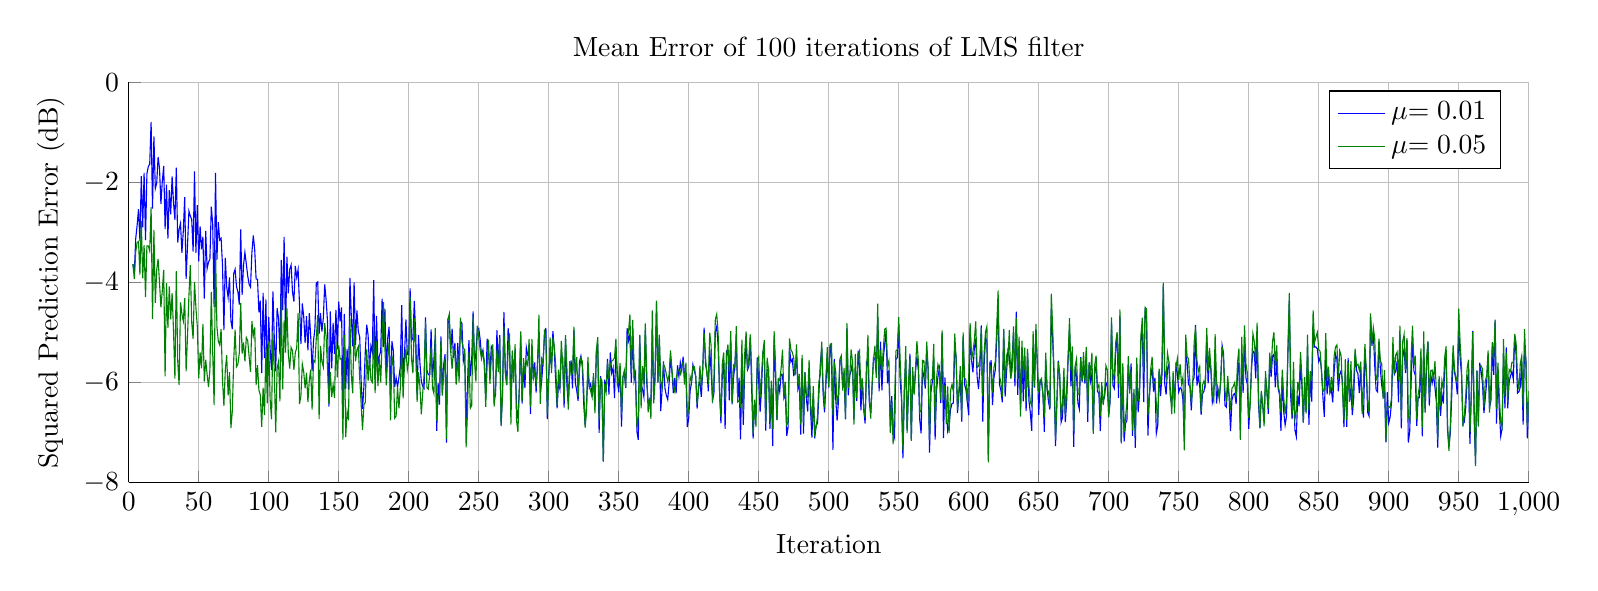
\begin{tikzpicture}

\begin{axis}[%
width=7in,
height=2in,
unbounded coords=jump,
scale only axis,
xmin=0,
xmax=1000,
xlabel={Iteration},
xmajorgrids,
ymin=-8,
ymax=0,
axis x line*=bottom,
axis y line*=left,
ylabel={Squared Prediction Error (dB)},
ymajorgrids,
title={Mean Error of 100 iterations of LMS filter},
legend style={draw=black,fill=white,legend cell align=left}
]
\addplot [color=blue,solid]
  table[row sep=crcr]{1	-inf\\
2	-inf\\
3	-3.63247548635504\\
4	-3.81027336542774\\
5	-3.12397691635872\\
6	-2.86119902064024\\
7	-2.53539684624931\\
8	-3.16676112268411\\
9	-1.87287963215152\\
10	-2.89688874222132\\
11	-1.80683447738346\\
12	-3.15464147007006\\
13	-1.82458327166948\\
14	-1.68218341073531\\
15	-1.63219789029952\\
16	-0.789873205247798\\
17	-2.52106072520631\\
18	-1.07635051731517\\
19	-2.12206374118726\\
20	-2.01047389834986\\
21	-1.49122357115496\\
22	-1.71447323590754\\
23	-2.42978853845123\\
24	-1.97543467466643\\
25	-1.67025813003234\\
26	-2.93089159099133\\
27	-2.04522139840017\\
28	-3.12381120028265\\
29	-2.15094901863687\\
30	-2.63505146356142\\
31	-1.87654503355272\\
32	-2.40262454377799\\
33	-2.7453475377885\\
34	-1.70088815294819\\
35	-3.19969168180634\\
36	-2.93538290069497\\
37	-2.81850679309292\\
38	-3.40593451015415\\
39	-2.97247798300073\\
40	-2.29111148470788\\
41	-3.92961782112619\\
42	-3.2598771586991\\
43	-2.57312199597864\\
44	-2.6698027618443\\
45	-2.73772306419399\\
46	-3.38216149089385\\
47	-1.7790567708878\\
48	-3.40601930425312\\
49	-2.45302270596887\\
50	-3.57691924870831\\
51	-2.87609797021169\\
52	-3.33570399128563\\
53	-3.08634697136012\\
54	-4.32247938157095\\
55	-2.96737516540653\\
56	-3.72326186941555\\
57	-3.59225336331484\\
58	-3.53905369715812\\
59	-2.48300424488342\\
60	-2.83484090695784\\
61	-4.49323109552297\\
62	-1.80790535669003\\
63	-3.54664196586379\\
64	-2.79275260967805\\
65	-3.15011448081517\\
66	-3.11598806703742\\
67	-3.6573829516309\\
68	-4.95268126957554\\
69	-3.50699770282685\\
70	-4.08799294216062\\
71	-4.29688941353878\\
72	-3.89856645447646\\
73	-4.76802800766952\\
74	-4.93285534162118\\
75	-3.81858257054167\\
76	-3.73662037444284\\
77	-4.08548666300303\\
78	-4.18449976039462\\
79	-4.44116335745449\\
80	-2.93965241749831\\
81	-4.24994426140523\\
82	-3.65904327453896\\
83	-3.39631035497168\\
84	-3.63029550539749\\
85	-3.86495830784621\\
86	-4.03579420976777\\
87	-4.09389458851054\\
88	-3.39546083627826\\
89	-3.06073325420393\\
90	-3.34518353549231\\
91	-3.9297234247452\\
92	-3.93591588076783\\
93	-4.59797380803468\\
94	-4.36193585400703\\
95	-5.81414545625924\\
96	-4.21003660536929\\
97	-5.51335235439191\\
98	-4.33995258796265\\
99	-5.94677100557913\\
100	-4.68788203220713\\
101	-5.32755486052862\\
102	-5.74994291163314\\
103	-4.17794058791482\\
104	-5.12754921609625\\
105	-5.77603347215157\\
106	-4.51314193359643\\
107	-4.71655557395317\\
108	-5.43301507578552\\
109	-3.54677166767047\\
110	-4.55415045099688\\
111	-3.08959662509114\\
112	-5.09745107089481\\
113	-3.4845546165726\\
114	-4.21639451783591\\
115	-3.73867758308483\\
116	-3.64946577428094\\
117	-4.19197457190497\\
118	-4.38341255737077\\
119	-3.66817467723873\\
120	-3.89816782030446\\
121	-3.7417274362719\\
122	-4.44215084486499\\
123	-5.23098015147528\\
124	-4.42082029417066\\
125	-4.67937965833079\\
126	-5.21045434660141\\
127	-4.672824558333\\
128	-5.3564470644181\\
129	-4.61557273509152\\
130	-5.07976867749425\\
131	-5.76993096063825\\
132	-5.17129559850032\\
133	-4.92355279811779\\
134	-4.01040597920574\\
135	-3.98708215533431\\
136	-5.03004173386208\\
137	-4.61598643906784\\
138	-4.98079675101542\\
139	-4.71236782097727\\
140	-4.04017591230564\\
141	-4.34323928682154\\
142	-4.77373668241086\\
143	-6.48527852730298\\
144	-4.57930871699374\\
145	-5.72007127207096\\
146	-4.81021375980704\\
147	-5.43180297652769\\
148	-4.54783620541458\\
149	-5.33590421980377\\
150	-4.38346842225619\\
151	-4.7798576259146\\
152	-4.49998366094842\\
153	-6.46597255074128\\
154	-4.62758413996881\\
155	-6.12279068351948\\
156	-5.32666086682675\\
157	-6.14326176489467\\
158	-3.90973747569214\\
159	-4.67608219325834\\
160	-5.27596721048848\\
161	-4.00001672868574\\
162	-5.24870722474813\\
163	-4.56010480853413\\
164	-4.97811546379956\\
165	-5.09200892830708\\
166	-5.95600299227652\\
167	-6.52910797356779\\
168	-6.07995648845875\\
169	-5.37865937100885\\
170	-4.84382308987329\\
171	-5.05247089781075\\
172	-5.74358097304372\\
173	-5.26927475423464\\
174	-5.38802607933097\\
175	-3.95085122606293\\
176	-5.92068981391143\\
177	-4.66673401104104\\
178	-5.64147466632448\\
179	-5.47439295810131\\
180	-5.36999949027796\\
181	-4.32344343362547\\
182	-5.29240310919425\\
183	-4.52825290402933\\
184	-5.83082814679367\\
185	-5.11532641306827\\
186	-4.88409276221222\\
187	-6.3077138762551\\
188	-5.17298461247613\\
189	-5.3640911771052\\
190	-6.08540688982492\\
191	-5.90709021487432\\
192	-6.08695057359163\\
193	-5.90276893050681\\
194	-5.68604302300088\\
195	-4.45463296698746\\
196	-5.93974876678861\\
197	-5.43835894566294\\
198	-4.73764074401358\\
199	-5.4402079607979\\
200	-5.44841981372918\\
201	-4.11656485851507\\
202	-5.1662958562123\\
203	-5.10160227378243\\
204	-4.36999677860943\\
205	-5.04048563983235\\
206	-6.25381252875435\\
207	-5.0525225863884\\
208	-5.60385206514297\\
209	-5.97558367999788\\
210	-6.07651272884729\\
211	-6.11757840630343\\
212	-4.70002008212081\\
213	-5.74929133900607\\
214	-5.84656722152092\\
215	-5.83647150154821\\
216	-4.93929297915624\\
217	-5.90126838173844\\
218	-5.5365048619832\\
219	-5.05437309425047\\
220	-6.96626179152201\\
221	-6.01192046341486\\
222	-6.44441141523838\\
223	-5.07908243300136\\
224	-6.2087930351626\\
225	-5.63483911726284\\
226	-5.43516055309898\\
227	-7.20392787829955\\
228	-4.7574906325865\\
229	-4.8091200696672\\
230	-5.40909432443294\\
231	-4.92424679703573\\
232	-5.5080526093555\\
233	-5.20897262479894\\
234	-6.02468654341483\\
235	-5.20617086110806\\
236	-5.65351642229129\\
237	-4.78684841727268\\
238	-4.81326665599696\\
239	-5.5743460697973\\
240	-5.41691249503153\\
241	-6.91370538446049\\
242	-6.061875839186\\
243	-5.1511316638344\\
244	-5.87464942024374\\
245	-5.53889277050666\\
246	-4.5763690643972\\
247	-5.64215698958383\\
248	-5.41075580221806\\
249	-4.9320763881816\\
250	-4.91606843154565\\
251	-5.13095840079967\\
252	-5.45146130304025\\
253	-5.35207893107668\\
254	-5.65180518705798\\
255	-6.30751990415229\\
256	-5.12596046613973\\
257	-5.37884763207993\\
258	-5.81388945073949\\
259	-5.28135623498713\\
260	-5.34922279060619\\
261	-6.33842907869098\\
262	-6.25235907711969\\
263	-4.95443440648462\\
264	-5.68182029936979\\
265	-5.05464073852348\\
266	-6.87084192509041\\
267	-6.18937261920408\\
268	-4.58688547993622\\
269	-5.71807902980792\\
270	-6.05382869171971\\
271	-4.91140917252148\\
272	-5.26549357281651\\
273	-6.46972242455554\\
274	-5.45705209273763\\
275	-5.79666221459682\\
276	-5.34593275536626\\
277	-6.51740719741179\\
278	-6.72466069670623\\
279	-6.13932469343251\\
280	-5.05736854302407\\
281	-6.42240688102698\\
282	-5.7034599544405\\
283	-6.11027609753542\\
284	-5.30015699496514\\
285	-5.45773976323318\\
286	-5.45951753936954\\
287	-6.62597504586006\\
288	-5.26611071094292\\
289	-5.93123064611013\\
290	-5.59673152155914\\
291	-6.20230995348154\\
292	-5.57926599795846\\
293	-4.97240123393268\\
294	-6.21535873184612\\
295	-5.96283713031937\\
296	-5.56194678124242\\
297	-5.06001676896531\\
298	-4.90789199114062\\
299	-6.73116244747968\\
300	-5.81765830569449\\
301	-5.45844721337095\\
302	-5.65755340892651\\
303	-4.97270753649066\\
304	-5.36137363291966\\
305	-5.98692057199177\\
306	-6.51646163144427\\
307	-5.99741160866835\\
308	-6.13053539214444\\
309	-5.44155725405102\\
310	-5.50452308514683\\
311	-6.50085636863276\\
312	-5.12032983757972\\
313	-6.06311931000256\\
314	-6.43278488252198\\
315	-5.79098173834879\\
316	-5.55919966611432\\
317	-6.11996122766985\\
318	-4.95132395774014\\
319	-6.00313422171055\\
320	-6.1602220348549\\
321	-6.36601816220336\\
322	-5.58457874882414\\
323	-5.47092689532269\\
324	-5.68519582545539\\
325	-6.4255179425403\\
326	-6.84869447531696\\
327	-6.46223434443977\\
328	-5.78387785337101\\
329	-6.09748999548839\\
330	-6.02537951398322\\
331	-6.28649029402066\\
332	-5.8893232604956\\
333	-6.49376301322322\\
334	-5.43193568637677\\
335	-5.2302407295576\\
336	-7.00570557536363\\
337	-5.87536850393572\\
338	-6.0921226487413\\
339	-7.58109655238898\\
340	-5.94432538638147\\
341	-6.18749105140354\\
342	-5.53029766925825\\
343	-6.24240935721256\\
344	-5.40091479696601\\
345	-5.81441215853284\\
346	-5.70699074077467\\
347	-6.31059951744851\\
348	-5.27973220765534\\
349	-5.825402471236\\
350	-6.19794906569978\\
351	-5.68930141253321\\
352	-6.88477706480699\\
353	-5.89966485442528\\
354	-5.80134058389781\\
355	-6.11231652828571\\
356	-4.91172358269061\\
357	-5.16701065451307\\
358	-5.03808445509694\\
359	-6.00178866570196\\
360	-4.97053891744597\\
361	-5.95606090873082\\
362	-5.8111968640196\\
363	-6.97962646432131\\
364	-7.14880859239347\\
365	-5.06203052550191\\
366	-6.03979792951178\\
367	-6.13740076009599\\
368	-6.28895286423998\\
369	-4.94711603784657\\
370	-6.00153211093415\\
371	-6.37783709932104\\
372	-6.35911309946962\\
373	-6.39520909302748\\
374	-4.91136267659422\\
375	-6.34196789836228\\
376	-5.78340049334494\\
377	-4.41686840319429\\
378	-6.00127234156922\\
379	-5.1141031730738\\
380	-6.57100194299706\\
381	-6.13634796443801\\
382	-5.58046130600922\\
383	-6.11080605597553\\
384	-6.25608900106351\\
385	-6.34280374332207\\
386	-6.01174976299095\\
387	-5.5059226256015\\
388	-5.77302797820211\\
389	-6.21174951131468\\
390	-5.91036142811176\\
391	-6.21643923907596\\
392	-5.65643602660234\\
393	-5.87625378558044\\
394	-5.60041980525291\\
395	-5.76400979970937\\
396	-5.48623029879221\\
397	-5.86728676096359\\
398	-5.81833247417846\\
399	-6.89375728075455\\
400	-6.71498490904695\\
401	-6.16610919326677\\
402	-6.01086063111315\\
403	-5.64430641252916\\
404	-5.7610198928047\\
405	-5.8740071045948\\
406	-6.52151622009926\\
407	-6.06152231702222\\
408	-5.99021615435154\\
409	-6.28909506034876\\
410	-5.75547907067113\\
411	-4.9055496271277\\
412	-5.64270422939714\\
413	-5.77462942933873\\
414	-6.17549397535771\\
415	-5.34637841579887\\
416	-5.77377750347591\\
417	-6.34638851094845\\
418	-6.22412640472565\\
419	-4.98395223421248\\
420	-4.88169346965297\\
421	-5.26053048186927\\
422	-6.13356387099421\\
423	-6.81881436562496\\
424	-5.85263847271346\\
425	-5.60710413751546\\
426	-6.92784871582064\\
427	-5.36885213210432\\
428	-5.35918219159089\\
429	-6.35851630662552\\
430	-5.15577455148012\\
431	-6.43602507341487\\
432	-5.91122540285455\\
433	-5.6364607465899\\
434	-5.07845149596862\\
435	-6.37044113491345\\
436	-5.90144383978427\\
437	-7.13619864648198\\
438	-5.66198560617958\\
439	-6.84829185614004\\
440	-5.69565184712314\\
441	-5.21038905448158\\
442	-5.74602603623736\\
443	-5.67009257552157\\
444	-5.09209003769615\\
445	-6.1675246236771\\
446	-7.12077860768153\\
447	-6.42466819342001\\
448	-6.69990301352987\\
449	-5.49662201089366\\
450	-5.98049972875489\\
451	-6.58643024206819\\
452	-6.12921408571996\\
453	-5.39509395956034\\
454	-5.41544679155032\\
455	-6.96305649540073\\
456	-5.74973808989141\\
457	-5.73245181455563\\
458	-6.92697545622467\\
459	-6.10803632933234\\
460	-7.27309401246576\\
461	-5.15295549463687\\
462	-5.87738095140143\\
463	-6.75307020766797\\
464	-6.02152277365841\\
465	-6.18464520202824\\
466	-5.83297861646135\\
467	-5.84932372358368\\
468	-6.30444044495689\\
469	-6.17590548351343\\
470	-7.06918035909515\\
471	-6.89692485437916\\
472	-5.30846902168894\\
473	-5.58900331463406\\
474	-5.53860472488627\\
475	-5.85581055966173\\
476	-5.824231791114\\
477	-5.42836883273495\\
478	-6.13011220102129\\
479	-6.01115286089343\\
480	-7.04310464274\\
481	-5.52677720408393\\
482	-7.02307572053903\\
483	-5.79245885749532\\
484	-6.31263365704206\\
485	-6.5796362012121\\
486	-5.72249696455865\\
487	-6.54520196499883\\
488	-7.10231720524289\\
489	-6.26403043413884\\
490	-7.1154193511289\\
491	-6.85659174833723\\
492	-6.81917188104063\\
493	-6.21711589062084\\
494	-5.63133979398266\\
495	-5.29742613307383\\
496	-6.22418579399263\\
497	-6.59700335852655\\
498	-6.03653967691978\\
499	-5.43612592270218\\
500	-6.10434269628614\\
501	-5.24781148954053\\
502	-5.44614687612927\\
503	-7.34982020200827\\
504	-5.52933568388819\\
505	-6.326675793077\\
506	-6.76137270260486\\
507	-6.34975967181399\\
508	-5.55628731536933\\
509	-5.55126236278956\\
510	-6.10512453934419\\
511	-5.85153771926865\\
512	-6.73355266489146\\
513	-4.91302522596299\\
514	-6.25872972120715\\
515	-5.85390798029895\\
516	-5.77280809618789\\
517	-5.58290923083379\\
518	-6.73796474761428\\
519	-5.70644620879392\\
520	-6.3736287267538\\
521	-5.36436900559163\\
522	-5.68746755609784\\
523	-6.5550990413794\\
524	-5.93868619227631\\
525	-6.54168525817138\\
526	-6.82207772560409\\
527	-5.58942137023265\\
528	-5.61769496870355\\
529	-6.39878300512966\\
530	-6.61913805174775\\
531	-6.07485612227207\\
532	-5.50421466224335\\
533	-5.53176848967398\\
534	-5.82703195479079\\
535	-4.70456273525146\\
536	-6.1757407373147\\
537	-5.18485455327379\\
538	-6.1577173589539\\
539	-5.51716832955581\\
540	-5.23061435828839\\
541	-4.97753355090464\\
542	-6.01773456763878\\
543	-5.75352745196735\\
544	-6.88782365157213\\
545	-6.27145004543987\\
546	-6.97837394995824\\
547	-7.09370339450926\\
548	-5.5387802014514\\
549	-5.50049085292688\\
550	-4.84650777288288\\
551	-5.95397129058524\\
552	-6.3353180058916\\
553	-7.51547425421538\\
554	-6.13481855566271\\
555	-5.53282017087052\\
556	-6.9648666470509\\
557	-6.13975448565191\\
558	-5.4256612607448\\
559	-7.14048150888861\\
560	-5.85376275210596\\
561	-6.21724854060614\\
562	-5.77983125934311\\
563	-5.48119846056152\\
564	-5.74963925638512\\
565	-6.74526801597326\\
566	-7.01956432446889\\
567	-5.73933004051956\\
568	-5.89546858283383\\
569	-6.1207004319744\\
570	-5.33657457805159\\
571	-5.72334895352998\\
572	-7.40248423469528\\
573	-6.18917061312388\\
574	-5.98896734506629\\
575	-5.53690506445108\\
576	-7.1423448284013\\
577	-6.16866788620437\\
578	-5.88939190353533\\
579	-5.72222344929627\\
580	-6.41439114053625\\
581	-5.00049349640505\\
582	-7.11397947690353\\
583	-5.90050928566835\\
584	-6.54157057669713\\
585	-6.97705568310344\\
586	-6.86589234475585\\
587	-6.54187499628816\\
588	-6.42457053504033\\
589	-6.4114230361077\\
590	-5.2962836083116\\
591	-5.48256717999719\\
592	-6.61257610730099\\
593	-6.21892756293227\\
594	-5.98489696384457\\
595	-6.78119317053104\\
596	-5.09762347320942\\
597	-6.04194978790732\\
598	-6.14200348359574\\
599	-6.39301384778108\\
600	-6.65464115971776\\
601	-4.92049914334566\\
602	-5.54606165066679\\
603	-5.79922750697102\\
604	-5.3126293645423\\
605	-5.13082944519888\\
606	-5.87982429928959\\
607	-6.12964211588444\\
608	-5.69893304294935\\
609	-4.86012151403314\\
610	-6.78352045181901\\
611	-5.65052200586308\\
612	-5.11120443841917\\
613	-5.18010399577664\\
614	-7.46115513923341\\
615	-5.77076495427348\\
616	-5.55195962584483\\
617	-6.4536510859213\\
618	-5.9094107059921\\
619	-5.74697458070801\\
620	-5.16448896436661\\
621	-4.42115670520035\\
622	-6.04444100975874\\
623	-6.16063773703088\\
624	-6.3971760546261\\
625	-4.96485998476704\\
626	-6.2818008267169\\
627	-5.80346282410655\\
628	-5.36852186001716\\
629	-5.48557382766632\\
630	-5.90725767955326\\
631	-5.50524692888851\\
632	-4.98825223627823\\
633	-6.07821252790799\\
634	-4.58292692799977\\
635	-6.24743901506482\\
636	-5.28734080682964\\
637	-6.54648862576565\\
638	-5.43079225105295\\
639	-6.37854840432809\\
640	-5.47255702376065\\
641	-6.57485270398749\\
642	-5.38154177452882\\
643	-6.36320790433887\\
644	-6.60145995975047\\
645	-6.9676278197242\\
646	-5.2671242270831\\
647	-6.10413190239755\\
648	-4.94343725239886\\
649	-5.63403617124845\\
650	-6.64741388989744\\
651	-5.9600876877849\\
652	-5.99428868444953\\
653	-6.215204867263\\
654	-6.98711499445259\\
655	-5.57496302756643\\
656	-6.12104217292177\\
657	-6.3885358935344\\
658	-6.54209218532554\\
659	-4.50656874627387\\
660	-5.16271177653041\\
661	-5.95144163777092\\
662	-7.27294818648587\\
663	-6.37520729304633\\
664	-5.56587182242826\\
665	-5.89742821364398\\
666	-6.79680628637358\\
667	-6.70075633402208\\
668	-5.91244030494851\\
669	-6.7898571057335\\
670	-6.36078535645132\\
671	-5.52681861022358\\
672	-4.92718885508284\\
673	-6.07813866828076\\
674	-5.50686174348645\\
675	-7.28600010188957\\
676	-5.68106953260364\\
677	-5.86564988205689\\
678	-6.41008778449587\\
679	-6.53007236475366\\
680	-5.49528827577776\\
681	-5.98898810332086\\
682	-5.65207691584034\\
683	-6.02222680964367\\
684	-5.36980001223721\\
685	-6.78814687966414\\
686	-5.59532519676297\\
687	-5.97896220781552\\
688	-5.82892077436857\\
689	-6.96104780539057\\
690	-5.78842561585208\\
691	-5.66406112254214\\
692	-6.18198332340876\\
693	-6.2212699513876\\
694	-6.97222331279329\\
695	-6.07312649574098\\
696	-6.35935335644909\\
697	-6.29811818483387\\
698	-5.99994111690564\\
699	-6.07349494340153\\
700	-6.65108013193634\\
701	-6.39605215951207\\
702	-4.8020983371306\\
703	-6.05896338436931\\
704	-6.12076358618913\\
705	-5.35084821349026\\
706	-5.01641896307579\\
707	-6.30641673241048\\
708	-4.66926820253325\\
709	-7.21702516194913\\
710	-5.69070486469849\\
711	-7.18083500878083\\
712	-6.81910823660167\\
713	-6.75864778401108\\
714	-5.63082222496552\\
715	-6.13650941143135\\
716	-5.61759027876267\\
717	-7.06606306822145\\
718	-6.22883022787847\\
719	-7.3094317332409\\
720	-5.6229116524459\\
721	-6.59544360424135\\
722	-6.23947722331583\\
723	-5.15606740095747\\
724	-4.91368054476909\\
725	-6.39370679885537\\
726	-4.5773779775305\\
727	-4.6704222889557\\
728	-7.06391356781721\\
729	-6.28407641013521\\
730	-5.89874137640082\\
731	-5.70102609961662\\
732	-6.18008516871105\\
733	-5.90595869962509\\
734	-7.02119115397125\\
735	-6.8657560728293\\
736	-5.76533304319806\\
737	-6.27281532018184\\
738	-5.88985225249343\\
739	-4.06180927276411\\
740	-6.02317773143197\\
741	-6.24353560941194\\
742	-5.72504418116686\\
743	-5.63703705932339\\
744	-6.27423759318624\\
745	-6.43993755837229\\
746	-5.92440212243077\\
747	-6.37262669720427\\
748	-5.67022599117987\\
749	-5.8031299207327\\
750	-6.19103204367608\\
751	-6.10373231711261\\
752	-6.13381674287752\\
753	-6.3440716500952\\
754	-7.18736487206945\\
755	-5.42165977900779\\
756	-5.60620274994066\\
757	-6.04298129383705\\
758	-6.0755807971432\\
759	-6.55775602332194\\
760	-5.96793230350398\\
761	-5.90488973840674\\
762	-4.85546147654366\\
763	-6.06306449112622\\
764	-5.88603569654181\\
765	-6.06322995837529\\
766	-6.6471843704442\\
767	-6.22286228496301\\
768	-6.17852469311027\\
769	-6.00195216928563\\
770	-5.08175273864688\\
771	-6.01850542899568\\
772	-5.48956675345489\\
773	-5.75585893040031\\
774	-6.39867781102939\\
775	-6.26901318082382\\
776	-5.39070889976995\\
777	-6.4199359376635\\
778	-6.12783147858921\\
779	-6.30152828440066\\
780	-5.97215155652648\\
781	-5.25719934624094\\
782	-5.41664963352518\\
783	-6.45789215338486\\
784	-6.49320472422084\\
785	-6.0380520200276\\
786	-6.28039142915391\\
787	-6.97252087648506\\
788	-6.35558595528997\\
789	-6.24361585566343\\
790	-6.21908359853896\\
791	-6.43003337941778\\
792	-5.82187673434182\\
793	-5.59603516534544\\
794	-6.96525734775948\\
795	-5.46105585032744\\
796	-6.20968034341986\\
797	-5.13727582302848\\
798	-5.90552528526303\\
799	-6.03527533083276\\
800	-6.92721378265264\\
801	-6.38928446326874\\
802	-5.70275570968429\\
803	-5.37242475341933\\
804	-5.40432598484521\\
805	-5.91520687225059\\
806	-5.04118151918686\\
807	-6.4186047873483\\
808	-6.9151814064783\\
809	-6.21950951453253\\
810	-6.46076483215274\\
811	-6.78620832107112\\
812	-5.90154750548747\\
813	-6.14595702023732\\
814	-6.62861889489512\\
815	-5.4987557472885\\
816	-5.89112451646117\\
817	-5.46974958851425\\
818	-5.4364573559944\\
819	-6.09912652648334\\
820	-5.52995688580734\\
821	-6.12380047237129\\
822	-6.24209330585443\\
823	-6.96688296896183\\
824	-5.87346617068868\\
825	-6.58380273040708\\
826	-6.85087903593208\\
827	-6.67327503388229\\
828	-5.40701945748833\\
829	-4.35529777335928\\
830	-6.2879449279998\\
831	-6.7332851421464\\
832	-6.04648883595409\\
833	-6.95293049780722\\
834	-7.08296821639256\\
835	-6.25895263082019\\
836	-6.47649843701908\\
837	-5.61626204444931\\
838	-6.06812249246004\\
839	-6.80441042314263\\
840	-6.00477608086912\\
841	-6.58643463191813\\
842	-5.27518037613553\\
843	-6.84596303196633\\
844	-5.82767073782714\\
845	-6.38196483328236\\
846	-4.83258739850024\\
847	-5.29055443521375\\
848	-5.28965261428229\\
849	-5.32733508629758\\
850	-5.5837292588711\\
851	-5.50019842414557\\
852	-5.75860672540543\\
853	-6.29663858921381\\
854	-6.68664172664437\\
855	-5.50987739754762\\
856	-6.23781737663835\\
857	-5.82768307134338\\
858	-6.21190294053101\\
859	-6.12792566925683\\
860	-6.39865768591369\\
861	-5.79650265267622\\
862	-5.43617623219487\\
863	-5.5404933675436\\
864	-6.17664360408119\\
865	-5.83914799113733\\
866	-5.76522228457586\\
867	-6.0052739236371\\
868	-6.89348034695299\\
869	-5.8040733108294\\
870	-6.88551982154821\\
871	-5.50750866587225\\
872	-6.37253499176539\\
873	-6.11351391209918\\
874	-6.65347726231413\\
875	-6.30281183111211\\
876	-5.40872722873813\\
877	-5.76057076548415\\
878	-5.82302733359215\\
879	-6.21183759723527\\
880	-5.69583560654253\\
881	-6.46312857378496\\
882	-6.70121447042562\\
883	-5.43626718531002\\
884	-5.79057738955141\\
885	-6.60246190881746\\
886	-6.6728246082295\\
887	-4.69196939523041\\
888	-5.26541710774586\\
889	-4.99060006628795\\
890	-5.66722501905019\\
891	-6.1507746180854\\
892	-6.18704964129023\\
893	-5.18070487409763\\
894	-5.71578347642196\\
895	-6.05751008475486\\
896	-6.25506070392434\\
897	-6.08260734848763\\
898	-7.19989565367109\\
899	-6.19236047420437\\
900	-6.80818100523333\\
901	-6.69337949049787\\
902	-6.39724448307126\\
903	-5.37226328676958\\
904	-5.83616006342821\\
905	-5.77180132265658\\
906	-5.57301173619454\\
907	-6.39534126778984\\
908	-5.03182477584246\\
909	-6.91790188120196\\
910	-5.47036126034754\\
911	-5.33025071943224\\
912	-5.81192717552259\\
913	-5.15238408612949\\
914	-7.20102593553571\\
915	-6.9778380630075\\
916	-6.00025787430672\\
917	-5.13935188020784\\
918	-5.76847839525113\\
919	-5.85778070825993\\
920	-6.86878302341119\\
921	-6.29979244702841\\
922	-6.30567729476315\\
923	-5.48177632827677\\
924	-7.07615802468135\\
925	-5.28468999021742\\
926	-6.58537790014163\\
927	-5.70220026986629\\
928	-5.19755927122354\\
929	-6.46104853081431\\
930	-5.84350792612125\\
931	-6.01540293733664\\
932	-5.84378455295344\\
933	-6.09386673180217\\
934	-6.37887084266446\\
935	-7.30440397819043\\
936	-5.92751461771309\\
937	-6.66615645427016\\
938	-6.22948009333059\\
939	-6.4214470906651\\
940	-5.69978200012693\\
941	-5.45649318497096\\
942	-6.94124698270518\\
943	-7.28921907678941\\
944	-7.00510346842878\\
945	-6.27243560878351\\
946	-5.41168322939593\\
947	-5.80442989121634\\
948	-5.95033557938057\\
949	-6.23872553607529\\
950	-4.91453347029086\\
951	-5.50315268885539\\
952	-5.84208870649835\\
953	-6.83759865217985\\
954	-6.79018976659876\\
955	-6.50432299641127\\
956	-5.96118683840667\\
957	-5.80793018159071\\
958	-7.2302249522258\\
959	-6.17696998717156\\
960	-4.97058125065142\\
961	-6.72691835097161\\
962	-7.62372507819108\\
963	-5.76007136797031\\
964	-6.80016805567325\\
965	-5.60648036291077\\
966	-5.77733391903957\\
967	-6.02830255308269\\
968	-6.61342201203019\\
969	-6.30124176722654\\
970	-5.97523651681753\\
971	-5.44051353859727\\
972	-6.49894726325563\\
973	-6.37288745284355\\
974	-5.27239879412615\\
975	-5.84727344887736\\
976	-4.7419570416948\\
977	-6.82102824699607\\
978	-5.80316235122179\\
979	-6.56987904385906\\
980	-7.07410782444692\\
981	-6.91770132847532\\
982	-5.42759795989927\\
983	-6.51573027047077\\
984	-5.30051049371916\\
985	-6.51835217068514\\
986	-5.98992697507144\\
987	-5.87158626693601\\
988	-5.77715192271757\\
989	-5.93822176679148\\
990	-5.06279559788093\\
991	-5.45235095708737\\
992	-6.21331208902013\\
993	-6.18582277676573\\
994	-6.08684895406409\\
995	-5.5778689960858\\
996	-6.84472303578738\\
997	-5.25312305571247\\
998	-5.54766143796934\\
999	-7.11900327277395\\
1000	-6.38300967321852\\
};
\addlegendentry{$\mu\text{ = 0.01}$};

\addplot [color=black!50!green,solid]
  table[row sep=crcr]{1	-inf\\
2	-inf\\
3	-3.63247548635504\\
4	-3.93028659363022\\
5	-3.38906828690839\\
6	-3.20096130844574\\
7	-3.1799134360866\\
8	-3.8411935954528\\
9	-2.76639402529972\\
10	-3.91646665987112\\
11	-3.25229787451263\\
12	-4.29230478496534\\
13	-3.2686520718288\\
14	-3.26778335594379\\
15	-3.36998270300881\\
16	-2.49072910880358\\
17	-4.72939513502913\\
18	-2.94863907720311\\
19	-4.4062529593115\\
20	-3.74882851815183\\
21	-3.52677260593842\\
22	-4.00509379579197\\
23	-4.49894850018756\\
24	-4.15786887366633\\
25	-3.74634518348942\\
26	-5.8759912333005\\
27	-4.01485849245513\\
28	-4.90700371212194\\
29	-4.07623403615972\\
30	-4.73756018446936\\
31	-4.21140775503519\\
32	-4.96554007423545\\
33	-5.92272997038101\\
34	-3.7735315490843\\
35	-5.57199863189526\\
36	-6.05353686941499\\
37	-4.39639913545874\\
38	-4.62891382672662\\
39	-4.77278588201405\\
40	-4.31182596731614\\
41	-5.77596260014775\\
42	-5.07738431935242\\
43	-4.26932702816833\\
44	-3.65540031457605\\
45	-4.80023416407126\\
46	-5.12812701148441\\
47	-3.9884074720239\\
48	-4.49906530291408\\
49	-4.87906754423568\\
50	-5.91758741804308\\
51	-5.39850783657477\\
52	-5.71577558205681\\
53	-4.82922907207079\\
54	-5.98059490885657\\
55	-5.54628081588448\\
56	-5.83959493917543\\
57	-6.09250462545014\\
58	-5.74234622327775\\
59	-4.18869478365115\\
60	-5.40484709948711\\
61	-6.45200706741968\\
62	-3.34849288436566\\
63	-4.88068689496432\\
64	-5.17317210728726\\
65	-5.25054554280326\\
66	-4.92877652466621\\
67	-5.95854684438848\\
68	-6.46504676207756\\
69	-5.75016641743878\\
70	-5.45602325071244\\
71	-6.26354896201767\\
72	-5.79379038385281\\
73	-6.9106790294446\\
74	-6.57517905451608\\
75	-5.54644451574626\\
76	-4.94452618807657\\
77	-5.68430160297296\\
78	-5.63348679557136\\
79	-5.40923731381229\\
80	-4.40854877598435\\
81	-5.42416794736867\\
82	-5.20097340024252\\
83	-5.57823942306281\\
84	-5.1026414280806\\
85	-5.16403271983014\\
86	-5.47833428143875\\
87	-5.78693839015873\\
88	-4.77322623076562\\
89	-5.06462916828914\\
90	-4.90087513356805\\
91	-6.0524016895811\\
92	-5.65326835005265\\
93	-6.15264052723612\\
94	-6.25218793883051\\
95	-6.88519384128132\\
96	-6.10514788638992\\
97	-6.65160099589965\\
98	-5.28948513416024\\
99	-6.41562550175724\\
100	-5.1848182567426\\
101	-6.3295611439698\\
102	-6.73711622899615\\
103	-5.00051433896939\\
104	-5.78680779496003\\
105	-6.9953621916114\\
106	-5.7255271373439\\
107	-5.57926128567525\\
108	-6.37610987216946\\
109	-4.29810968247667\\
110	-6.13738807042615\\
111	-4.76056476217393\\
112	-5.40171721836983\\
113	-4.51452854325378\\
114	-5.4241436018158\\
115	-5.7219943534307\\
116	-5.30000992072075\\
117	-5.36552853916528\\
118	-5.74657624021885\\
119	-5.40516414429055\\
120	-5.30847041723988\\
121	-4.61388747282615\\
122	-6.43195788277837\\
123	-6.26589858739295\\
124	-5.63172662664294\\
125	-5.78662445868094\\
126	-6.11817619523031\\
127	-5.8054515638521\\
128	-6.39137999177725\\
129	-5.95541138763851\\
130	-5.74407625116906\\
131	-6.54267326505262\\
132	-5.5570630188789\\
133	-5.59532305323589\\
134	-5.11231891265407\\
135	-4.64779688152717\\
136	-6.73186347472795\\
137	-5.27093215106855\\
138	-5.58083441785007\\
139	-5.68849649272279\\
140	-4.81316052872865\\
141	-5.08443111221023\\
142	-5.7243221558005\\
143	-6.42695107724219\\
144	-5.7881540267467\\
145	-6.28953774750333\\
146	-6.046525837989\\
147	-6.30861723778736\\
148	-5.17671686757354\\
149	-5.89628685985926\\
150	-5.26088164364936\\
151	-5.53182543191309\\
152	-5.52338308995265\\
153	-7.14348322672885\\
154	-5.05514508380267\\
155	-7.09226274918771\\
156	-6.57543110099485\\
157	-6.75542759503891\\
158	-4.70416215750174\\
159	-5.84879518911445\\
160	-6.2149492439014\\
161	-4.80604466627498\\
162	-5.57605043819629\\
163	-5.34814391918209\\
164	-5.28339030848275\\
165	-5.91575130331175\\
166	-6.41885544093523\\
167	-6.9476827793233\\
168	-6.44602955033633\\
169	-6.39756779982259\\
170	-5.33708557151544\\
171	-5.96976968717156\\
172	-5.50077597499423\\
173	-5.94845843315887\\
174	-5.99435711500244\\
175	-4.97981226533619\\
176	-6.21023532888442\\
177	-5.17934320500473\\
178	-6.0739461492384\\
179	-5.51688416548997\\
180	-5.99821203338332\\
181	-5.17287186194709\\
182	-4.39507160475776\\
183	-5.30558636485493\\
184	-6.05721317844931\\
185	-5.48245686317639\\
186	-5.20162545217404\\
187	-6.75769836702351\\
188	-5.46816455948428\\
189	-5.6488512920295\\
190	-6.71263559201828\\
191	-6.67257859895918\\
192	-6.08919768069271\\
193	-6.51532150130253\\
194	-6.11732782327673\\
195	-5.26754959053784\\
196	-6.31763560786637\\
197	-5.62593893981551\\
198	-5.32303318827253\\
199	-5.74824372840492\\
200	-5.57074330041876\\
201	-4.29264954197771\\
202	-5.51976186769202\\
203	-5.81471166165186\\
204	-4.71099451274104\\
205	-5.36479049706896\\
206	-6.38652125338454\\
207	-5.79250764289614\\
208	-6.08056981228341\\
209	-6.63882547588169\\
210	-6.20582820788112\\
211	-5.85495334776362\\
212	-4.77835101822168\\
213	-6.10321765194908\\
214	-6.13461222687554\\
215	-5.84085969094865\\
216	-5.29028521908322\\
217	-6.11651087035858\\
218	-6.21942108563248\\
219	-4.90896219360925\\
220	-6.76301994507341\\
221	-6.28417116999555\\
222	-6.26068756515912\\
223	-5.17062149740987\\
224	-6.26106646131888\\
225	-5.79465756147862\\
226	-5.5103116995975\\
227	-7.13259730357938\\
228	-4.74173784723353\\
229	-4.62815609679215\\
230	-5.38639702868585\\
231	-5.72862369462379\\
232	-5.32342147520553\\
233	-5.40864093527106\\
234	-6.04337500987364\\
235	-5.4234012754691\\
236	-5.99862369880349\\
237	-4.70515998224652\\
238	-5.18271514834428\\
239	-5.31846677137453\\
240	-5.3387819869259\\
241	-7.29830969475388\\
242	-6.59090104968567\\
243	-5.39076769524529\\
244	-6.51355842689069\\
245	-6.45722717174225\\
246	-4.66499732161625\\
247	-5.58631123981486\\
248	-5.98453595373271\\
249	-4.86299526128202\\
250	-5.08839764470929\\
251	-5.34251790991858\\
252	-5.52862045768518\\
253	-5.40358993176455\\
254	-5.56569691970412\\
255	-6.48854911020409\\
256	-5.66102002844479\\
257	-5.14138548467787\\
258	-6.02930782958613\\
259	-5.50243874530256\\
260	-5.23753113213983\\
261	-6.48352342811788\\
262	-6.15729129569109\\
263	-5.34677446317179\\
264	-5.79048249323311\\
265	-5.10605963237236\\
266	-6.85105697208859\\
267	-6.2576213562575\\
268	-4.88460710620218\\
269	-5.82063592648956\\
270	-6.04928940164222\\
271	-5.37281078415232\\
272	-5.01786969325577\\
273	-6.84172961115941\\
274	-5.35800862352387\\
275	-6.00184690037139\\
276	-5.23351015386096\\
277	-6.75887313492874\\
278	-6.98958693902922\\
279	-6.11980835715528\\
280	-4.97946820651366\\
281	-6.38321950162158\\
282	-5.51557356267781\\
283	-5.83999087944659\\
284	-5.57332454305296\\
285	-5.65476008539224\\
286	-5.12861883387384\\
287	-6.49160346936828\\
288	-5.12928183737135\\
289	-5.93119996255456\\
290	-5.77365569509358\\
291	-6.02437001662445\\
292	-5.75492350797365\\
293	-4.64077640357965\\
294	-6.42796251820205\\
295	-5.53193141845575\\
296	-5.62122622995074\\
297	-4.93907024008317\\
298	-5.12131071299591\\
299	-6.63389364097133\\
300	-6.00060051770233\\
301	-5.09855214615357\\
302	-5.81499985522088\\
303	-5.10018400914629\\
304	-5.28014422930329\\
305	-5.65492192317133\\
306	-6.46824427907184\\
307	-5.74173248916851\\
308	-6.11103191726202\\
309	-5.16635551396545\\
310	-5.66109787772452\\
311	-6.36162242986769\\
312	-5.05373715899431\\
313	-5.70669599904397\\
314	-6.54052703964541\\
315	-5.57417513578825\\
316	-5.84775072885496\\
317	-5.81723100183329\\
318	-4.88463505251648\\
319	-5.87759078014643\\
320	-5.49422116047703\\
321	-6.29281502575405\\
322	-5.74146699452987\\
323	-5.50896029857559\\
324	-5.58106254212158\\
325	-6.1276205462382\\
326	-6.90856847097983\\
327	-6.56523367616754\\
328	-5.48962155051877\\
329	-6.08360256456374\\
330	-6.17439747850582\\
331	-6.29342463516783\\
332	-5.81143536248141\\
333	-6.61948803315967\\
334	-5.35907962758249\\
335	-5.0953618233182\\
336	-6.75462552403279\\
337	-5.92637791488926\\
338	-5.95159790571864\\
339	-7.57773157165751\\
340	-6.0284267737595\\
341	-6.1847899087875\\
342	-5.58711341464893\\
343	-5.93721936413093\\
344	-5.63614327588569\\
345	-5.56884377927382\\
346	-5.55168015265179\\
347	-5.50489054740723\\
348	-5.1218441926151\\
349	-6.05985377002998\\
350	-5.94122166395532\\
351	-5.61027271232337\\
352	-6.64224909226435\\
353	-5.89122401384132\\
354	-5.76219789929538\\
355	-6.09645515602992\\
356	-5.10810143102098\\
357	-4.99149166836158\\
358	-4.6369233454911\\
359	-5.810015284363\\
360	-4.75049980588401\\
361	-5.72972793713423\\
362	-6.01342418732489\\
363	-6.89224937588026\\
364	-6.66967412640513\\
365	-5.04992430424433\\
366	-6.51789965930254\\
367	-5.67438226154878\\
368	-6.04320168406527\\
369	-4.82027023287258\\
370	-5.78468733725886\\
371	-6.59652534065219\\
372	-6.3023580827541\\
373	-6.72610679844042\\
374	-4.55763308595753\\
375	-6.41820038746309\\
376	-5.92495652937932\\
377	-4.36501494757262\\
378	-5.9901639028614\\
379	-5.04253347209522\\
380	-5.95411983400138\\
381	-6.14650107397097\\
382	-5.6360811093538\\
383	-5.69787794528265\\
384	-5.8365150626281\\
385	-5.97351180195757\\
386	-5.844710257992\\
387	-5.35625632240741\\
388	-5.73270890653683\\
389	-6.0635835841632\\
390	-6.17781443595822\\
391	-5.93095046078075\\
392	-5.77010472023429\\
393	-5.74740471563124\\
394	-5.83039016081993\\
395	-5.66604323280414\\
396	-5.58908357990671\\
397	-6.04264404133993\\
398	-5.60331445162795\\
399	-6.65648429835236\\
400	-6.53334332208733\\
401	-5.88246242871298\\
402	-5.97262933854433\\
403	-5.67734314061533\\
404	-5.68284999122\\
405	-5.87600037654668\\
406	-6.42859464384797\\
407	-6.18446287225419\\
408	-5.66303025619161\\
409	-6.0925460368697\\
410	-5.74332847191535\\
411	-5.00386003509483\\
412	-5.49200551993999\\
413	-5.85115071007591\\
414	-5.97240045419217\\
415	-5.00171090860704\\
416	-5.2624344806738\\
417	-6.40207495140768\\
418	-5.96927840468635\\
419	-4.74023322400755\\
420	-4.63507387777104\\
421	-5.00381714101035\\
422	-6.17042404335095\\
423	-6.68784663241705\\
424	-5.61935380527209\\
425	-5.40128240165315\\
426	-6.37370032317437\\
427	-5.46114636379135\\
428	-5.24121934257796\\
429	-5.78444786617469\\
430	-4.97209745511821\\
431	-6.41873536783142\\
432	-5.65792812818747\\
433	-5.71456362569001\\
434	-4.87471407187461\\
435	-6.38843528177793\\
436	-6.36587238857671\\
437	-6.46276884178346\\
438	-5.14092128455536\\
439	-6.56769886581439\\
440	-5.42128240503571\\
441	-4.97933241221514\\
442	-5.74804367158861\\
443	-5.48974199682965\\
444	-5.03604147377067\\
445	-5.82402310077988\\
446	-7.0356737752283\\
447	-6.34158631101927\\
448	-6.89028683966744\\
449	-5.57707258554958\\
450	-5.49134462365718\\
451	-6.3084085575177\\
452	-5.86623094542331\\
453	-5.38665300691802\\
454	-5.15357037168962\\
455	-6.82461324453152\\
456	-5.5060007998698\\
457	-5.74458328983247\\
458	-6.80172761320365\\
459	-5.96142320466536\\
460	-6.930615649499\\
461	-4.97319213184024\\
462	-5.6367431618746\\
463	-6.75168562168689\\
464	-5.92552573090754\\
465	-5.95953368366395\\
466	-5.71896009344645\\
467	-5.34455135727099\\
468	-6.30098977253259\\
469	-5.98676010836151\\
470	-6.84469950734206\\
471	-6.7946707622873\\
472	-5.11967930141948\\
473	-5.34411207876749\\
474	-5.39712921940337\\
475	-5.51027449327236\\
476	-5.85795731456803\\
477	-5.24003744795011\\
478	-6.08316928928071\\
479	-5.82691783110199\\
480	-6.8410772181253\\
481	-5.44968652356577\\
482	-6.80027212981801\\
483	-5.80381276021738\\
484	-6.23703839087407\\
485	-6.28609516052754\\
486	-5.55006691516171\\
487	-6.42781321408049\\
488	-6.79649437782634\\
489	-6.07438096419925\\
490	-7.02530497107201\\
491	-6.89765875344098\\
492	-6.67469811812074\\
493	-5.98475244003762\\
494	-5.83413643691855\\
495	-5.1830109254646\\
496	-6.10082585756462\\
497	-6.5043979608508\\
498	-5.88995958227335\\
499	-5.29108293970541\\
500	-6.08847933965578\\
501	-5.23415616504779\\
502	-5.22074998158755\\
503	-6.65725833764168\\
504	-5.59079685624723\\
505	-5.7880021617467\\
506	-6.45972691839284\\
507	-6.23428263914631\\
508	-5.52967694858582\\
509	-5.46294967697815\\
510	-6.16258931522255\\
511	-5.70600377185205\\
512	-6.73558423269785\\
513	-4.81268080182964\\
514	-6.10632323809382\\
515	-5.88278327007862\\
516	-5.33809594338888\\
517	-5.5886992130418\\
518	-6.84256713598646\\
519	-5.42977980207468\\
520	-6.31429875777884\\
521	-5.45779321873851\\
522	-5.36978924489867\\
523	-6.150081698073\\
524	-5.91650181178095\\
525	-6.516595827787\\
526	-6.70397482501084\\
527	-5.82083772302\\
528	-5.04775223885885\\
529	-6.27706355317956\\
530	-6.72035271285915\\
531	-6.02552601975344\\
532	-5.53567913965799\\
533	-5.26525701921673\\
534	-5.90681960454679\\
535	-4.42315804028319\\
536	-6.03121288662977\\
537	-5.35317241974999\\
538	-5.74800650770961\\
539	-5.33011429229877\\
540	-4.93455691398944\\
541	-4.91447228969348\\
542	-5.6615844538492\\
543	-5.56298926154845\\
544	-7.0095474521566\\
545	-6.40335873680481\\
546	-7.23809651474918\\
547	-6.45894626303098\\
548	-5.36872465338449\\
549	-5.34219034834719\\
550	-4.69231621684581\\
551	-5.53282880571985\\
552	-6.20384684943003\\
553	-7.35633883473333\\
554	-6.24369611466348\\
555	-5.27235327548684\\
556	-7.012170434665\\
557	-6.00448347951426\\
558	-5.50587960916488\\
559	-7.16564469461746\\
560	-5.69162548789179\\
561	-6.24659450068298\\
562	-5.69537833835544\\
563	-5.17409567671141\\
564	-5.55613731121989\\
565	-6.60130701102982\\
566	-6.55624457261674\\
567	-5.55636960753658\\
568	-5.56691931168428\\
569	-6.05252769873087\\
570	-5.18310338139509\\
571	-5.75097829187053\\
572	-7.15455098375893\\
573	-5.95436437888354\\
574	-5.93188682184704\\
575	-5.22692470630446\\
576	-6.8507785994459\\
577	-5.92943739681736\\
578	-5.63866590066761\\
579	-5.73944629434624\\
580	-6.34044888907391\\
581	-4.95743211652241\\
582	-6.35466863004721\\
583	-6.05401021176321\\
584	-6.82955403584135\\
585	-6.07711067738446\\
586	-7.00572655566685\\
587	-6.16819344588398\\
588	-6.04361770772923\\
589	-6.1773031530508\\
590	-5.02381811472531\\
591	-5.52937039870785\\
592	-6.54750100601017\\
593	-6.13713310072378\\
594	-5.6745808939588\\
595	-6.69730289142347\\
596	-4.99635697447382\\
597	-5.8983594204968\\
598	-5.95189226489729\\
599	-6.38282598463267\\
600	-5.88733530781338\\
601	-4.80582497528732\\
602	-5.55851285408657\\
603	-5.38515937193273\\
604	-5.16891898656483\\
605	-4.77948825151057\\
606	-5.69746133092272\\
607	-5.67671584552079\\
608	-5.53009621176655\\
609	-4.90929741374868\\
610	-6.27454891900721\\
611	-5.40703904116442\\
612	-4.98375471755275\\
613	-4.87714865343094\\
614	-7.59602982371947\\
615	-5.64473952041322\\
616	-5.740162612411\\
617	-6.20452046174781\\
618	-5.70189861978897\\
619	-5.58007025811907\\
620	-4.90054612750469\\
621	-4.15729869980721\\
622	-5.87662694981446\\
623	-5.99581613329106\\
624	-6.28480547243039\\
625	-4.93064007397269\\
626	-6.0869335455701\\
627	-5.47236107238725\\
628	-5.58000056362545\\
629	-4.95413823556496\\
630	-5.92392707738455\\
631	-5.75696818964248\\
632	-4.88044057231006\\
633	-5.92393329593107\\
634	-4.70873012372333\\
635	-5.93480983743014\\
636	-5.08357942332395\\
637	-6.68154221705505\\
638	-5.16201070163297\\
639	-5.89972002174614\\
640	-5.30196146361057\\
641	-6.39101062048673\\
642	-5.32638372306104\\
643	-6.07205718545351\\
644	-6.3916309037621\\
645	-6.46800869973346\\
646	-4.97133066686741\\
647	-6.07956014586864\\
648	-4.82987233440812\\
649	-5.65364536056483\\
650	-6.19148034553884\\
651	-5.96437726066616\\
652	-5.91838475388117\\
653	-6.26310661250183\\
654	-6.68763419740371\\
655	-5.40534678373126\\
656	-6.17000284187596\\
657	-6.17015299084768\\
658	-6.49815089396344\\
659	-4.22163475543978\\
660	-4.95060255716629\\
661	-5.82354621160925\\
662	-7.1490141647365\\
663	-6.36440591951567\\
664	-5.58934487810438\\
665	-5.82855583879681\\
666	-6.68689225992693\\
667	-6.4105194080316\\
668	-5.709413367781\\
669	-6.65081383023675\\
670	-6.11332887006041\\
671	-5.46495412816876\\
672	-4.71519577288705\\
673	-5.76104263786249\\
674	-5.27792965759137\\
675	-6.96906951709955\\
676	-5.67336118139914\\
677	-5.52548187827282\\
678	-6.23468190699898\\
679	-6.2285265849171\\
680	-5.50837841756515\\
681	-5.97041276025986\\
682	-5.391406529636\\
683	-5.96091622570025\\
684	-5.28731192440322\\
685	-6.59008739566561\\
686	-5.6162075841487\\
687	-5.80772169290789\\
688	-5.40561782865922\\
689	-7.03006329068556\\
690	-5.65110615951542\\
691	-5.46221976389082\\
692	-6.1161706898285\\
693	-6.04381981187845\\
694	-6.67298195479291\\
695	-5.99348574136147\\
696	-6.45111175487409\\
697	-6.23388372591678\\
698	-5.66242584165242\\
699	-5.74690065715783\\
700	-6.69573618077221\\
701	-6.24890201993783\\
702	-4.69785698077559\\
703	-5.94141110432571\\
704	-5.83956016021874\\
705	-5.19943097287898\\
706	-4.99341390038106\\
707	-6.03387920008117\\
708	-4.53883690387239\\
709	-7.21370856068222\\
710	-5.62013668809679\\
711	-6.99879898418084\\
712	-6.6947068497483\\
713	-6.39633195774015\\
714	-5.47295160330164\\
715	-6.22082007239608\\
716	-5.73808706042804\\
717	-6.96160587450194\\
718	-6.13042393165102\\
719	-7.06618712225473\\
720	-5.50403026035324\\
721	-6.37600856905886\\
722	-6.13886558790766\\
723	-5.05856668185674\\
724	-4.70423967475019\\
725	-5.81812300117436\\
726	-4.49628293464721\\
727	-4.53008949738241\\
728	-6.65531114522112\\
729	-6.31361832636617\\
730	-5.73781508259243\\
731	-5.48624662997832\\
732	-6.00491744339459\\
733	-5.99086430496594\\
734	-6.41500606592412\\
735	-6.82015867493568\\
736	-5.72292880811772\\
737	-6.03025861081665\\
738	-5.76522458706118\\
739	-4.00455222433747\\
740	-5.76207207761783\\
741	-5.91719530668553\\
742	-5.41116388887857\\
743	-5.59054537143651\\
744	-6.1390006078111\\
745	-6.6316247690785\\
746	-5.77122596003607\\
747	-6.61614968753283\\
748	-5.70711008479336\\
749	-5.52405202546012\\
750	-5.94694143443767\\
751	-5.63219783571938\\
752	-6.03283513090458\\
753	-5.89955883899268\\
754	-7.3600621011199\\
755	-5.04175188437213\\
756	-5.48580852822626\\
757	-5.52702585011345\\
758	-6.00472658174301\\
759	-6.39942599133785\\
760	-6.06542983050804\\
761	-5.2103598823698\\
762	-4.88509514216085\\
763	-5.54714875447414\\
764	-5.7837995459444\\
765	-5.68450025838079\\
766	-6.5924421815783\\
767	-6.05229321879372\\
768	-5.97195962634801\\
769	-6.06118453251648\\
770	-4.90801495078162\\
771	-5.77790222915293\\
772	-5.30745654533061\\
773	-5.7139192991729\\
774	-6.22446701802018\\
775	-6.36935611869619\\
776	-5.03171533503317\\
777	-5.98415770729337\\
778	-6.13736868983684\\
779	-6.33705408345045\\
780	-5.93377883901677\\
781	-5.28331570084091\\
782	-5.50455429374762\\
783	-6.16096270459305\\
784	-6.38672650056958\\
785	-5.87078025315294\\
786	-6.24951089073152\\
787	-6.55381916072723\\
788	-6.11693990769837\\
789	-6.07679535077539\\
790	-6.00094229723747\\
791	-6.30057344588479\\
792	-5.60159483833861\\
793	-5.31858815902145\\
794	-7.14719164585224\\
795	-5.08942423987352\\
796	-6.07239281515549\\
797	-4.86039983226244\\
798	-5.62629898925025\\
799	-5.80465446162941\\
800	-6.70854608205477\\
801	-6.47743489644375\\
802	-5.67504801137447\\
803	-5.0237183597929\\
804	-5.19118347705379\\
805	-5.57456667588992\\
806	-4.80298686209419\\
807	-6.24869958397606\\
808	-6.91062014956192\\
809	-6.17050664830787\\
810	-6.41832337629369\\
811	-6.87603046369322\\
812	-5.77183335834645\\
813	-6.23325883193248\\
814	-6.52206264997515\\
815	-5.40272169695974\\
816	-5.7571797847221\\
817	-5.18085687176554\\
818	-4.99657398457151\\
819	-5.67802877863164\\
820	-5.25839554655521\\
821	-6.0606105141337\\
822	-6.19566785651049\\
823	-6.60211020285837\\
824	-5.74250765492219\\
825	-6.30450307607547\\
826	-6.63803502547035\\
827	-6.33786122947384\\
828	-5.36520675685763\\
829	-4.2077473051404\\
830	-5.99331577448285\\
831	-6.66237392871289\\
832	-5.58964797065416\\
833	-6.73061096303248\\
834	-6.575138129698\\
835	-5.98973446924564\\
836	-6.17362906272891\\
837	-5.38869214805438\\
838	-5.91020259095259\\
839	-6.7976623021212\\
840	-5.89257149233636\\
841	-6.62037109469007\\
842	-5.04255746507602\\
843	-6.55459992896915\\
844	-5.77515575111877\\
845	-5.96075449471416\\
846	-4.55793171274441\\
847	-5.1996522687669\\
848	-5.0940278966292\\
849	-4.99756131246302\\
850	-5.34306569592927\\
851	-5.37781463003903\\
852	-5.7959503996915\\
853	-6.18462282086781\\
854	-6.14383870462319\\
855	-5.01128146292335\\
856	-5.93542028027266\\
857	-5.68268347697106\\
858	-6.20852366321391\\
859	-5.89143005355032\\
860	-6.16347714497382\\
861	-5.47309767516281\\
862	-5.29049102581269\\
863	-5.24855424584709\\
864	-5.91982381905808\\
865	-5.36568393153528\\
866	-5.46311784295249\\
867	-6.16636793006016\\
868	-6.75818671845297\\
869	-5.53391347564989\\
870	-6.75285015109044\\
871	-5.58183130765702\\
872	-6.38707519571036\\
873	-5.57094189123107\\
874	-6.50440194579031\\
875	-5.9736578231201\\
876	-5.32440172225187\\
877	-5.65962409937391\\
878	-5.63543698761517\\
879	-5.76014054996418\\
880	-5.58465016125692\\
881	-6.62666792575261\\
882	-5.9670844494285\\
883	-5.22775199534656\\
884	-5.76261497034633\\
885	-6.40744931298454\\
886	-6.59779650684784\\
887	-4.62012676666544\\
888	-5.21126550748183\\
889	-4.90253761056738\\
890	-5.11594309841888\\
891	-5.94550618478716\\
892	-5.8775052615175\\
893	-5.1213186798841\\
894	-5.56166279039743\\
895	-5.62809155645284\\
896	-6.33153192152873\\
897	-5.75220427466908\\
898	-7.17778718599759\\
899	-6.47498516476959\\
900	-6.47898357337839\\
901	-6.50216944612636\\
902	-6.31810402621487\\
903	-5.09384371142588\\
904	-5.81990983141076\\
905	-5.45169929332449\\
906	-5.39179793262328\\
907	-5.95924299881413\\
908	-4.86417368016471\\
909	-6.71219587731814\\
910	-5.17847550378635\\
911	-5.03668213645224\\
912	-5.74657112206068\\
913	-5.11513190554455\\
914	-6.67849603376611\\
915	-6.76203660613203\\
916	-5.48304313670217\\
917	-4.86153897798083\\
918	-5.65520395085313\\
919	-5.46233598059453\\
920	-6.73527691645987\\
921	-6.24976316712089\\
922	-6.06624420230873\\
923	-5.31876316538438\\
924	-6.90339651306718\\
925	-4.97758501399815\\
926	-6.6066082540127\\
927	-5.53006492601161\\
928	-5.17427187310979\\
929	-6.31972054776047\\
930	-5.77148820583899\\
931	-5.75089013813251\\
932	-5.96872922839419\\
933	-5.57533220441805\\
934	-6.14864686581875\\
935	-7.14157817348208\\
936	-5.86843974824657\\
937	-6.47216903350106\\
938	-5.96260689774716\\
939	-6.11890295781318\\
940	-5.48791401487863\\
941	-5.27530085158415\\
942	-6.82529972288808\\
943	-7.3717960908712\\
944	-6.84919987927695\\
945	-5.92736796333695\\
946	-5.25215403795965\\
947	-5.75376850769133\\
948	-5.89975785727876\\
949	-5.99162820061981\\
950	-4.52167036385749\\
951	-5.20733233572743\\
952	-5.71211576365983\\
953	-6.88315270261402\\
954	-6.65671258736002\\
955	-6.26729837303491\\
956	-5.7203713546614\\
957	-5.54644822923989\\
958	-6.99583256198536\\
959	-6.27571603852632\\
960	-4.99283623827519\\
961	-6.37711828686763\\
962	-7.67283906689512\\
963	-5.77300928118847\\
964	-6.88269950109849\\
965	-5.67856801135173\\
966	-5.66912274262413\\
967	-5.72819917009222\\
968	-6.50021693706518\\
969	-5.96350172067787\\
970	-5.87036495215411\\
971	-5.35901304003534\\
972	-6.60192520270683\\
973	-6.01304940700091\\
974	-5.1913915201153\\
975	-5.52575956342705\\
976	-4.76133335146358\\
977	-6.52622079694873\\
978	-5.6031549476047\\
979	-6.30110277143637\\
980	-6.79005479322692\\
981	-6.89056094771211\\
982	-5.1308496237242\\
983	-6.2756668344064\\
984	-5.40530012304561\\
985	-6.39158908410223\\
986	-5.74107902487566\\
987	-5.77968434290063\\
988	-5.59805489372102\\
989	-5.60548862414435\\
990	-5.02857873989449\\
991	-5.21545043407324\\
992	-5.89250603013219\\
993	-6.14250331028649\\
994	-5.61773796753751\\
995	-5.47010785643005\\
996	-6.48613879569587\\
997	-4.93464712199502\\
998	-5.60336993970241\\
999	-6.88934802581138\\
1000	-6.1694282114741\\
};
\addlegendentry{$\mu\text{ = 0.05}$};

\end{axis}
\end{tikzpicture}%}
   	\caption{\textit{LMS filter error (dB) for the given AR process, averaged over 100 independent trials}}
   	\label{fig:q3_1_b}
\end{figure}


\subsubsection{Misadjustment} \label{sec:3_1_c}

Misadjustment is defined as $ \mathcal{M} = \frac{\mathrm{EMSE}}{\sigma^2_\eta}$, where the total mean squared error $ \mathrm{MSE} = \lim_{n \to \infty} \mathbb{E} \{ e^2 (n) \} = \sigma^2_\eta + \mathrm{EMSE} $. Thus we can compute the measured misadjustment from the known mean squared error, and variance of the White Gaussian Noise. We also know that we can approximate $  \mathcal{M} \approx \frac{\mu}{2} \mathbf{Tr} \{ \mathbf{R} \}$ (for small $\mu$) which allows us to have an idea of its theoretical values.

Based on the data obtained in section \ref{sec:3_1_b}, we have taken the mean error squared of the last two hundred samples (when it is known to be in a steady state) across the 100 iterations of the LMS filter, and computed the misadjustment. Table \ref{tab:3_1_c} shows the theoretical and measured misadjustment values. The results are close to the theoretical values, although running the test multiple times does show that the misadjustment varies between each set of 100 trials.

\begin{table}[h]
\centering
\begin{tabular}{|l|l|l|}
\hline	
$\mu$  & Theoretical $\mathcal{M}$ & Measured $\mathcal{M}$ \\ \hline
0.01 & 0.0093                    & 0.0028                 \\ \hline
0.05 & 0.0463                    & 0.0456                 \\ \hline
\end{tabular}
\caption{\textit{Theoretical and Actual Misadjustment values measured for different step sizes}}
\label{tab:3_1_c}
\end{table}

\subsubsection{Steady State Coefficient Values}
By taking the mean of the two hundred last values (when we know the filter is in steady state), and then taking the mean across 100 iterations, we can get estimations of the coefficients $a_1$ and $a_2$. The results are shown in table \ref{tab:3_1_d}. We can see that the coefficient estimates for $\mu = 0.01$ is nearer to the true values than for $\mu = 0.05$. We know that there will always be some error, due to the power of the WGN signal (the $ \sigma^2$ term in the Mean Squared Error equation). We also know from section \ref{sec:3_1_c} that the misadjustment for  $\mu = 0.05$ is larger than for $\mu = 0.01 $, hence it is not surprising that it also less close to the known values than  $\mu = 0.01$. However, we know that a larger step size results in faster convergence to the correct value, so it is a case of a trade off between a small steady state error, and fast convergence.

\begin{table}[h]
\centering
\begin{tabular}{|l|l|l|l|}
\hline
$\mu$ & True Values & 0.05   & 0.01   \\ \hline
$a_1$ & 0.1               & 0.0689 & 0.0943 \\ \hline
$a_2$ & 0.8               & 0.7176 & 0.7691 \\ \hline
\end{tabular}
\caption{\textit{Theoretical and Actual Coefficient values measured for different step sizes}}
\label{tab:3_1_d}
\end{table}

\subsubsection{Leaky LMS Derivation}
In order to derive the leaky LMS equation, we differentiate the given cost function, using the known result of $ \nabla ( e^2(n) ) |_{w_n}$, and that $ \nabla (\lVert \mathbf{x}(n)\rVert_2^2 )|_{x_n} = 2\mathbf{x} $  :

\begin{subequations}
\begin{align}
J(n) &= \frac{1}{2} ( e^2(n) + \gamma \lVert \mathbf{w}(n) \rVert_2^2 ) \\
\nabla J(n)|_{w_n} &= \frac{1}{2}  ( \nabla ( e^2(n) ) |_{w_n} + \gamma \nabla (\lVert \mathbf{w}(n)\rVert_2^2 )|_{w_n} ) \\
\nabla J(n)|_{w_n} &= -e(n) \mathbf{x}(n) + \gamma w(n)
\end{align}
\end{subequations}

We then substitute this in to the update function:

\begin{subequations}
\begin{align}
\mathbf{w}(n+1) &= \mathbf{w}[n] + \mu (- \nabla J(n)|_{w_n}) \\
\mathbf{w}(n+1) &= \mathbf{w}[n] + \mu e(n) \mathbf{x}(n) - \mu \gamma \mathbf{w}(n) \\
\mathbf{w}(n+1) &= (1 - \mu \gamma ) \mathbf{w}[n] + \mu e(n) \mathbf{x}(n)
\end{align}
\end{subequations}



\subsubsection{Leaky LMS Results}

Table \ref{tab:3_1_f} shows estimated parameters for $a_1$ and $a_2$ with varying $\mu$ (the same values used in section \ref{sec:3_1_b}) and $\gamma$ values. We can see that as the leakage parameter $\gamma$ increases, the coefficient estimates get progressively less accurate. \cite{Kamenetsky2004} defines $ \lim_{n \to \infty } \mathbb{E}[\mathbf{w}_n] = (\mathbf{R} + \gamma \mathbf{I})^{-1} \mathbf{p} $. The new term added is the $\gamma \mathbf{I} $ term, which effectively introduces noise in to the input matrix $ \mathbf{x} $. Its purpose is to allow the input matrix to have non-zero eigenvalues, as in some cases this can happen, meaning coefficients do not converge. Since the extra term is effectively adding white noise, this explains why the coefficient estimates get progressively worse as $ \gamma $ increases. Since the purpose of Leaky LMS is to help coefficients converge if they otherwise cannot, care should be taken when to add the $ \gamma $ term in, and when it is used to keep it as small as possible, so as to ensure the most accurate results are obtained.

\begin{table}[h]
\centering
\begin{tabular}{|l|l|l|}
\hline
               & $\mu = 0.01 $                  & $\mu = 0.05 $                  \\ \hline
$\gamma = 0$   & $a_1 = 0.0939$, $a_2 = 0.7694$ & $a_1 = 0.0695$, $a_2 = 0.7162$ \\ \hline
$\gamma = 0.2$ & $a_1 = 0.1320$, $a_2 = 0.6078$ & $a_1 = 0.1043$, $a_2 = 0.5463$ \\ \hline
$\gamma = 0.5$ & $a_1 = 0.1412$, $a_2 = 0.4682$ & $a_1 = 0.1105$, $a_2 = 0.4110$ \\ \hline
$\gamma = 0.8$ & $a_1 = 0.1349$, $a_2 = 0.3836$ & $a_1 = 0.1050$, $a_2 = 0.3333$ \\ \hline
\end{tabular}
\caption{\textit{Estimated AR Coefficients for different $\mu$ and $\gamma$}}
\label{tab:3_1_f}
\end{table}

\subsection{Adaptive Step Sizes}

\subsubsection{Implemented GASS Algorithms}

\subsubsection{NLMS Algorithm}

The NLMS algorithm is a modification to the LMS algorithm which normalises the power of the input, which for a noisy input signal means the filter is more likely to be stable.

\begin{subequations}
	\begin{align}
	\bigtriangleup \mathbf{w}(n) &= \mathbf{w}(n+1) - \mathbf{w}(n) \\
	\bigtriangleup \mathbf{w}(n) &= \mu e(n) \left[  1 - \mu \frac{\lVert \mathbf{x}(n)\rVert^2}{1 + \mu \lVert \mathbf{x}(n)\rVert^2} \right] \mathbf{x}(n) = \mathbf{w}(n+1) - \mathbf{w}(n) \\
	\bigtriangleup \mathbf{w}(n) &= e(n) \left[ \frac{\mu + \mu^2  \lVert \mathbf{x}(n)\rVert^2 - \mu^2 \lVert \mathbf{x}(n)\rVert^2}{1 + \mu \lVert \mathbf{x}(n)\rVert^2} \right] \mathbf{x}(n) = \mathbf{w}(n+1) - \mathbf{w}(n) \\
	\mathbf{w}(n+1) &= \mathbf{w}(n) + \left[ \frac{1}{\frac{1}{\mu} + \mathbf{x}^T(n)\mathbf{x}(n) } \right] e(n) \mathbf{x}(n)  \label{subeq:3_2_b}
	\end{align}
\end{subequations}

We can see that the last line, equation \ref{subeq:3_2_b} now has the same form (and thus is equivalent to, other than the factors which are discussed below) as the NLMS update equation:
$$ \mathbf{w}(n+1) = \mathbf{w}(n) + \frac{\beta}{\epsilon + \mathbf{x}^T(n)\mathbf{x}(n)} e(n) \mathbf{x}(n) $$

Thus from the comparison of forms, we can determine that $ \beta = 1 $ and $ \epsilon = \frac{1}{\mu} $.

\subsubsection{GNGD Algorithm}



%  \begin{figure}[h]
%  	\centering 
% 	\resizebox{0.6\textwidth}{!}{\input{q5/q5_cum.tikz}}
%   	\caption{\textit{Cumulative representation of the variance of each eigenvector}}
%   	\label{fig:q5_4}
%  \end{figure}

% \begin{figure}[h]
% 	\centering 
%  	\setlength\figureheight{0.4\textwidth}
% 	\setlength\figurewidth{0.7\textwidth} 
%  	\input{p_1/1.tikz}
%  	\caption{\textit{The four randomly generated subsets}}
%  	\label{fig:q1}
% \end{figure}


%  \begin{figure}[h]
%          \centering
%          \begin{subfigure}[b]{0.45\textwidth}
%             \resizebox{\textwidth}{!}{\input{part_4/q8_num_1.tikz}}
%   			\caption{\textit{1 Tree}}
%          \end{subfigure}
%          ~ %add desired spacing between images, e. g. ~, \quad, \qquad, \hfill etc.
%           %(or a blank line to force the subfigure onto a new line)
%          \begin{subfigure}[b]{0.45\textwidth}
%             \resizebox{\textwidth}{!}{\input{part_4/q8_num_3.tikz}}
%   			\caption{\textit{2 Trees}}
%          \end{subfigure}
 		
%          \begin{subfigure}[b]{0.45\textwidth}
%             \resizebox{\textwidth}{!}{\input{part_4/q8_num_5.tikz}}
%   			\caption{\textit{5 Trees}}
%          \end{subfigure}
%          ~ %add desired spacing between images, e. g. ~, \quad, \qquad, \hfill etc.
%           %(or a blank line to force the subfigure onto a new line)
%          \begin{subfigure}[b]{0.45\textwidth}
%             \resizebox{\textwidth}{!}{\input{part_4/q8_num_10.tikz}}
%   			\caption{\textit{10 Trees}}
%          \end{subfigure}
         
%          \begin{subfigure}[b]{0.45\textwidth}
%             \resizebox{\textwidth}{!}{\input{part_4/q8_num_20.tikz}}
%   			\caption{\textit{20 Trees}}
%          \end{subfigure}
 		
%  		\label{q9i}
% 		\caption{\textit{Varying the Number of Trees in the Forest}}
%  \end{figure}

\end{document}

